\cotefile{156-1}
\scanpage{1}
\figure{
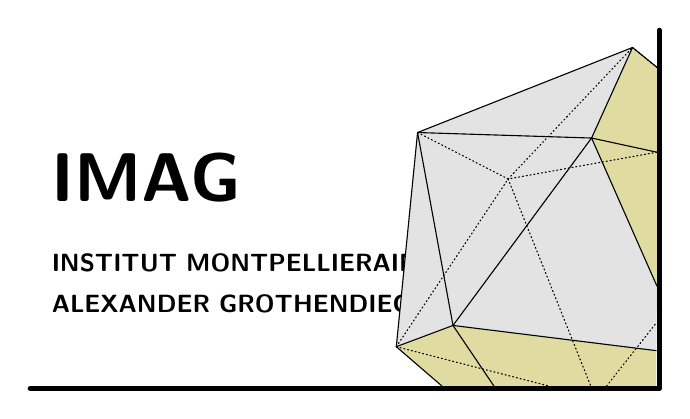
\begin{tikzpicture}[x=1cm,y=1cm,line join=round,line cap=round]
\node[anchor=west,font=\sffamily\bfseries\fontsize{40}{44}\selectfont] at (-4.5,2.65) {IMAG};
\node[anchor=west,font=\sffamily\bfseries\fontsize{9}{11}\selectfont] at (-4.5,1.56) {INSTITUT MONTPELLIERAIN};
\node[anchor=west,font=\sffamily\bfseries\fontsize{9}{11}\selectfont] at (-4.5,1.05) {ALEXANDER GROTHENDIECK};
\coordinate (A) at (0,0.50);
\coordinate (B) at (0.27,3.22);
\coordinate (C) at (3.00,4.30);
\coordinate (D) at (3.32,4.04);
\coordinate (E) at (3.31,2.97);
\coordinate (F) at (3.31,1.27);
\coordinate (G) at (3.30,0.00);
\coordinate (H) at (0.58,0.00);
\coordinate (I) at (0.72,0.77);
\coordinate (J) at (2.48,3.15);
\coordinate (K) at (1.42,2.63);
\fill[gray!22] (A)--(B)--(C)--(J)--(F)--(G)--(H)--cycle;
\fill[olive!28] (C)--(D)--(E)--(J)--cycle;
\fill[olive!28] (J)--(E)--(F)--cycle;
\fill[olive!28] (A)--(I)--(3.30,0.45)--(G)--(H)--cycle;
\draw (A)--(B)--(C)--(D);
\draw (C)--(J)--(F);
\draw (B)--(J)--(E);
\draw (B)--(I)--(1.24,0);
\draw (A)--(I)--(J);
\draw (I)--(3.30,0.45);
\draw[densely dotted] (A)--(K)--(C);
\draw[densely dotted] (B)--(K)--(E);
\draw[densely dotted] (K)--(2.47,0);
\draw[densely dotted] (A)--(1.94,0);
\draw[densely dotted] (2.67,0)--(3.30,0.80);
\draw[densely dotted] (C)--(D);
\draw (A)--(H);
\draw[line width=1.8pt] (-4.65,-0.03)--(3.34,-0.03)--(3.34,4.52);
\end{tikzpicture}
}

\scanpage{2}
\mspage{1}
\margin{\unsure{Ch|Cf} I}

Vers une géométrie des formes (topologiques)

(\uline{Juin \unsure{86}})

\margin{(5 juin)}
Approche vers une construction récurrente (sur l'entier naturel $n$) d'une ``géométrie des formes de dimension $\leq n$''.

Une \deleted{\unsure{``espace''}} ``forme de dim 0'' sera par définition un ensemble discret dont les éléments sont appelés les ``lieux'' de la forme.

\margin{Un modèle d'une forme de dim 0 sera un ens. $L$ (``lieux'') avec une relation d'équivalence (``non disjoints''). La forme \unsure{du} modèle est l'ens quotient.}

\uline{\deleted{\unsure{Formes}}\inserted{Modèle} de dimension 1}

Un \deleted{tel} tel modèle comporte

\deleted{
\textcircled{1} Un ensemble des ``\uline{lieux}'' de la forme, $L$.

\textcircled{2} Un sous-ensemble $L_0$ de $L$, formé des lieux dits ``\uline{critiques}'' ou ``\uline{de branchement}''.

3) Une relation \inserted{symétrique} dans $L$ (i.e. $R\subset L\times L$) ``$x$ et $y$ sont \uline{disjoints}'', impliquant la relation ``$x$ et $y$ sont distincts''.

4) Une relation \inserted{symétrique} plus fine ``$x$ et $y$ sont \uline{adjacents}''

\textcircled{5} Une \deleted{ensemble de parties de $L$, (appelés \inserted{\unsure{comme support}} ``\uline{segments}'' \unsure{``$x$ est s}} \inserted{\unsure{S} relation plus fine encore} (\unsure{comme ci dessus} pas symétrique) ``$x$ \deleted{\unsure{est}} est spécialisation de $y$'' (qui implique que $x$ est critique, et $y$ n'est pas critique).

\textcircled{6} Un ensemble $S$, \deleted{\unsure{partition de $L$}, \inserted{dont les éléments, \unsure{``segments''}}} \unsure{appelés} ``\uuline{segments}''

\textcircled{7} Pour tout segment \deleted{\unsure{un}} $I$, deux parties $\unsure{\delta I|\partial I}$ de
}
\rotatebox{90}{\reflectbox{\unsure{EXTRA STRONG}}}

\rotatebox{90}{\reflectbox{\unsure{EXTRA STRONG}}}
\mspage{1}

\scanpage{3}
\deleted{
deux éléments de $L$ (\uline{adjacents} l'un de l'autre) \inserted{appelés ``lieux \unsure{extrémals|extrémales} du segment''}

\textcircled{8} Une partie $\tilde I$ de $L$ (l'ens des lieux de $\mathcal X$. \uline{sur} le segment) contenant $\delta I$.

\uline{NB} 1) Si $x,y\in L$, alors $x,y$ sont adjacents sss $\exists I\in S$ tel que $\{x,y\}=\delta I$. Donc, la donnée (4) \deleted{est inutile} résulte des autres (dans 7) il faut dire que si $\delta I=\{x,y\}$, $x$ et $y$ sont disjoints\ldots)

2) Je présume que si $x,y\in L$ sont adjacents, il y aura au plus deux segments $I$ tels que $\delta I=\{x,y\}$. (il y en aura effectivement deux sss $x,y$ appartiennent à une ``composante connexe'' de $\mathcal X$ qui est un (modèle d'un) cercle.

3) Je ne sais s'il faut supposer que $I$ est \unsure{connue} quand on connaît $\delta I$ et $\tilde I$, i.e. si on peut \deleted{définir par \unsure{le|un}} \inserted{$S\subset\unsure{\mathcal P}_2(\unsure{L_0|L})\times\unsure{\mathcal P}(L)$}

\uline{Axiomes} \inserted{\unsure{supplém.}} (à voir)

\deleted{On dit que la forme est de dim 0}

\margin{\deleted{\unsure{*}}}
$\unsure{E_1|E_2}$ Dans $L_0$, la relation ``$x$ et $y$ ne sont \uline{pas} disjoints'' est une relation d'équivalence.

L'ensemble quotient est appelé l'ens des \uline{points} \inserted{critiques, ou de branchement} de la forme.
\deleted{(\unsure{de})}
(\deleted{\unsure{NB}} plusieurs lieux critiques \unsure{différents} peuvent définir le même point critique)
}
\rotatebox{90}{\reflectbox{\unsure{EXTRA STRONG}}}

\rotatebox{90}{\reflectbox{\unsure{EXTRA STRONG}}}

\mspage{2}

\scanpage{4}
\mspage{2}
\deleted{\unsure{Deux} \unsure{1)} Un ensemble $L$ (l}

1) Deux ensembles de base $\unsure{L|L_*}$ (ensemble des \uline{lieux} du modèle) et $S$ (ensemble des \uline{segments} du modèle)

2) Une application $\unsure{S}\longrightarrow\mathcal P(L)$, $I-\tilde I$ (lieux sur un \unsure{segment}) -- i.e. une relation entre $S$ et $L$.

3) Une application $\delta:S\longrightarrow\mathcal P_2(L)$, \inserted{$I\longmapsto\delta I$,} telle que $\delta I\subset\tilde I$.

\deleted{\unsure{1}} $+$ axiomes

\uline{NB} J'ignore s'il faut supposer que $I$ est connu, quand on connaît $\tilde I$ et $\delta I$, i.e. s'il faut supposer $I\longrightarrow\mathcal P(L)\times\mathcal P_2(L)$ injectif.

\margin{7.6. On verra que $I$ est connu quand on connaît $\tilde I$, on identifie $I$ \unsure{à $\tilde I$}, et $S$ à une partie de $\mathcal P(L)$.}

Si $I$ est un segment, les éléments de $\delta I$ sont les lieux extrémités, et ceux de $\tilde I\setminus\delta I$ \inserted{$=\deleted{\unsure{\delta I}}\tilde I^\circ$} sont les lieux intérieurs au segment.

Un lieu est dit \uline{régulier} s'il est intérieur à \inserted{(au moins)} un segment, \uline{singulier} (\deleted{\unsure{ou}} critique, lieu de branchement) sinon.
\[
L_r=\bigcup_{I\in S}(\tilde I\setminus\delta I),\qquad L_s=L\setminus L_r
\]
Ainsi, pour tout $I\in S$, on a
\[
\tilde I\cap L_s\subset\delta I
\]
\mspage{3}

\rotatebox{90}{\reflectbox{\unsure{EXTRA STRONG}}}
\rotatebox{90}{\reflectbox{\unsure{EXTRA STRONG}}}

\scanpage{5}
\mspage{3}
Soient $x,y\in L$, on dit que $y$ est une \uline{spécialisation} de $x$ si \deleted{$\unsure{\exists}$}

a) $y$ est singulier, et b) $\exists I\in S$ tel que $x\in\tilde I^\circ$, $y\in\delta I$.

\deleted{
\uline{Axiomes}\deleted{\unsure{s}}

$F_1)$ Soit $I\in S$, alors \deleted{$\unsure{\exists}$} $\tilde I^\circ$ ($\underset{\text{déf}}{=}\tilde I\setminus\delta I$) est non vide, et si $z\in\tilde I^\circ$, \deleted{$\unsure{\exists}$} $\delta I=\{x,y\}$,
\[
\exists!\ I_{x,z}\in S,\ I_{y,z}\in S\quad\text{tels que}
\]
\[
\tilde I_{x,z},\tilde I_{y,z}\unsure{\in|\subset}\tilde I,\qquad
\delta I_{x,z}=\{x,z\},\quad\delta I_{y,z}=\{y,z\}.
\]
De plus, on a alors
\[
\tilde I_{x,z}\cap\tilde I_{y,z}=\{z\}
\]
}
\margin{décomposition des segments

\uuline{décomposition} des segments

Mais attention, je ne dis pas que $\tilde I=\tilde I_{x,z}\cup\tilde I_{y,z}$ !!!}
\margin{Ajouter: $\forall\unsure{\tilde J|J}\in S$ tel que $\tilde J\subset\tilde I$, $\delta\tilde J\ni z$, on a $\tilde J\subset\tilde I_{x,z}$ ou $\tilde J\subset\tilde I_{y,z}$. \deleted{\unsure{Alors}} \deleted{\unsure{il}}}

\deleted{
$F_2)$ \deleted{Soient $x,y$ lieux réguliers. Alors, \unsure{il} existe $I\in S$ tel que $x,y\in\tilde I^\circ$, alors}
\inserted{Soient $I\in S$, et \deleted{$\unsure{x,y}$} $\unsure{\Phi|\varphi}\in\tilde I^\circ$}
$\exists$ \deleted{$\unsure{I\in S}$} $I'\in S$ tel que
a) \deleted{$\unsure{x}$} $\unsure{\Phi|\varphi}\in\tilde I'^\circ$,
b) $\tilde I'\subset\tilde I^\circ$.

\inserted{\uline{Corollaire 1} $\tilde I$ est \uline{infini}.

\uline{Corollaire 2} Si $S\neq\varnothing$, $S$ est \uline{infini}\ldots
(car l'ens des $\unsure{\tilde J|J}\in S$ tels que $\tilde J\subset\tilde I$ est infini\ldots)}

\deleted{$\unsure{F_2}$} $F_2)$ (Réciproque de $F_1$) Soient $I',I''\in S$, tels que
\[
\tilde I'\cap\tilde I''=\deleted{\unsure{\{z\}}}\delta I'\cap\delta I''=\{z\},
\]
avec $z$ \uline{régulier}. Alors $\exists!\ I\in S$, tel que
\[
\tilde I'\cup\tilde I''\subset\tilde I\deleted{\unsure{*}}
\quad\text{et}\quad
\delta I=(\delta I'\cup\delta I'')\setminus\{z\},
\]
et on \inserted{a, si $\delta I'=\{x,z\}$, $\delta I''\deleted{\unsure{=}}\ =\{y,z\}$, $\unsure{I'|\tilde I'}=\tilde I_{x,z}$, $\unsure{I''|\tilde I''}=\tilde I_{y,z}$.}

\deleted{$F_3)$ Soit $x\in\unsure{L}$}
\inserted{\unsure{cf plus bas}}

$F_3)$ Soit $I\in S$, $\Phi$ partie finie de $\tilde I^\circ$,
Alors $\exists I'\in S$ tel que $\tilde I^\circ\supset\tilde I'\supset\Phi$.
}
\margin{\uuline{recollement} des segments}
\margin{\uuline{\unsure{Filtration}}}
\margin{\deleted{\unsure{l'ens des} $\tilde I$ \unsure{tels que} $x\in\tilde I^\circ$ \unsure{est filtrant}, si on a $x\in\tilde I'^\circ\cap\tilde I''^\circ$,
$\exists\tilde I$ tel que
$x\in\tilde I^\circ\subset\tilde I'^\circ\cap\tilde I''^\circ$.
Il en résulte qu'il \unsure{existe} $I$, \unsure{avec}
\deleted{$\unsure{\tilde I\subset\tilde I'^\circ}$}
$\tilde I\subset\tilde I'^\circ\cap\tilde I''^\circ$,
$x\in\tilde I^\circ$.}}
\mspage{4}

\rotatebox{90}{\unsure{EXTRA STRONG}}
\rotatebox{90}{\unsure{EXTRA STRONG}}

\scanpage{6}
\mspage{4}
\uline{Modèle d'une forme 1-dimensionnelle}

$L$, ensemble des ``\uline{lieux}''

$S$, \rule{3cm}{0.4pt} ``segments''

\[
S\longrightarrow\mathcal P(L),\qquad I\longmapsto\tilde I
\quad(\tilde I,\text{ ens des lieux \uline{sur} le segment }I)
\]
\[
S\longrightarrow\mathcal P_2(L)\qquad I\longmapsto\delta I
\quad(\delta I,\text{ ens des deux lieux \uline{extrémités} de }I)
\]
avec $\delta I\subset\tilde I$

$F_1)$ \unsure{Soient|Soit} $I\in S$, $\delta I=\{x,y\}$. \deleted{\unsure{Alors deux}}

[Soit $S_{I,x}$ l'ens des $J\in S$ tels que $\tilde J\subset\tilde I$, $\delta J\ni x$, et soit
$S_{I,x}\longrightarrow\tilde I\setminus\{x\}$ définie par
$J\longmapsto z$ tel que $\delta J=\{x,z\}$. Cette application est bijection, i.e.]
$\forall z\in\tilde I\setminus x$, $\exists!\ J\in S$, \deleted{\unsure{un}} soit $I_{x,z}$ tel que
\[
\unsure{\tilde J_{x,z}|\tilde I_{x,z}}\subset\tilde I,\qquad
\unsure{\delta J_{x,z}|\delta I_{x,z}}=\{x,z\}
\]
\margin{axiome de décomposition}
\margin{NB $I_{x,y}=I_{y,x}=I$}

\deleted{De plus, on a si $z\in\tilde I^\circ$ (i.e. $z\in\tilde I\setminus\{x,y\}$),}
\inserted{$F_2)$ Soit $I\in S$, alors $\tilde I^\circ\neq\varnothing$, et si $z\in\tilde I^\circ$,}
\deleted{on a}
\[
\tilde I_{x,z}\cap\tilde I_{y,z}=\{z\}.
\]
\margin{(\unsure{7.6.|6.6.}) \unsure{Faudra|Faut} \unsure{indiquer} qu'on \unsure{fait sauter|fait passer} la condition de divisibilité $\tilde I^\circ\neq\varnothing$.}

Si $J\in S$ est tel que $\tilde J\subset\tilde I$, $z\in\delta J$,
on a $\tilde J\subset\tilde I_{x,z}$ \uline{ou} $J\subset\tilde I_{y,z}$.

\uline{Cor. 1} \deleted{$\unsure{\forall}$} $\forall I\in S$, $\tilde I^\circ$ est infini [du fait de la condition de divisibilité)

\uline{Cor. 2} Dans $F_2$, les relations $\tilde J\subset\tilde I_{x,z}$ et $\tilde J\subset\tilde I_{y,z}$ sont exclusives l'une de l'autre.

\uline{Cor 3} Soit $I\in S$, \deleted{$\unsure{\exists}$} $S_I=\{J\in S\mid\tilde J\subset\tilde I\}$, et
\[
S_I\unsure{-|\longrightarrow}\mathcal P_2(\tilde I)\qquad J\longmapsto\delta J.
\]
Alors \deleted{\unsure{cette}}

a) Cette application est injective.

b) Son image contient les $\varepsilon\in\mathcal P_2(\tilde I)$ tels que $\varepsilon\cap\delta I\neq\varnothing$.
\mspage{5}

\rotatebox{90}{\reflectbox{\unsure{EXTRA STRONG}}}
\rotatebox{90}{\reflectbox{\unsure{EXTRA STRONG}}}

\scanpage{7}
\mspage{5}
c) Si $\{u,v\}\in\mathcal P_2(\tilde I)$ tel que $\{u,v\}\cap\delta I=\varnothing$
(i.e. $\{u,v\}\in\mathcal P_2(\tilde I^\circ)$) alors conditions équivalentes

\unsure{1)} \deleted{\unsure{donc}} $\exists J\in S_I$ tel que $\delta J=\{u,v\}$

2) On a $v\in\tilde I_{x,u}$ \uline{ou} $v\in\tilde I_{y,u}$

3) On a $u\in\tilde I_{y,v}$ ou $u\in\tilde I_{x,v}$

\margin{\uline{NB} de \unsure{$=$|c}
\[
v\in\tilde I_{x,u}\Longleftrightarrow u\in\tilde I_{y,v}
\]
\[
v\in\tilde I_{y,u}\Longleftrightarrow u\in\tilde I_{x,v}
\]
\deleted{\unsure{Cela vaut pour} \unsure{$u,v\in\tilde I^\circ$}}
\deleted{\unsure{la condition de disjonction}}
\deleted{\unsure{$u\in\tilde I^\circ$, $v\in\tilde I^\circ$}}
\unsure{vaut} si on \deleted{\unsure{$u,v\in\tilde I$}} \unsure{suppose} que \deleted{\unsure{$u\neq v$}} $u,v\in\tilde I$ (quelconques, \unsure{supposons} $u,v\in\tilde I^\circ$ mais $u\neq v$)}

[\uline{NB} on dit alors que $u$ et $v$ sont \inserted{des lieux} \uline{disjoints} sur le segment $I$ -- on y reviendra\ldots]

\uline{Cor. 4} Si $\tilde I=\tilde J$ alors $I=J$ [donc on peut identifier $S$ à une partie de $\mathcal P(L)$]

$F_3)$ Soient $I,J\in S$, \inserted{$x\in L$} tels que $x\in\delta I\cap\delta J$.

Alors, \deleted{ou bien $\exists\unsure{z}\in I^\circ\cap J^\circ$ tel que $I_{x,z}=J_{x,z}$, ou bien} \deleted{$\unsure{\exists}$}
$\exists\unsure{u}\in I^\circ$, $v\in J^\circ$ tels que \deleted{$\unsure{I_{x,}}$} l'on ait
\[
\left\{
\begin{array}{l}
I_{x,u}=J_{x,v}\quad(\text{donc }u=v\text{ et }u=v\in I^\circ\cap J^\circ)\\
\uline{\text{ou}}\quad \tilde I_{x,u}\cap\tilde J_{x,v}=\{x\}
\end{array}
\right.
\]
\margin{\uline{Axiome des branches}}
\margin{Voir \unsure{renforcement} $F_3'$ \unsure{aussi} p.\ 10 et \deleted{\unsure{20}}}
\margin{écrire plutôt $u\in I\setminus\{x\}$, $v\in J\setminus\{x\}$ (si on n'admet pas condition de divisibilité) \deleted{\unsure{pour $I$}}}

\uline{NB} Ces deux relations sont mutuellement exclusives.

\deleted{La première, est}
La condition
\[
\exists z\in\tilde I^\circ\cap\unsure{\tilde J^\circ|J^\circ}
\quad\text{tel que}\quad
\unsure{I_{x,z}=I_{y,z}|I_{x,z}=J_{x,z}}
\]
est une relation \uline{d'équivalence} \inserted{$R_x$} dans l'ens \inserted{$S_x$} des segments $I\in S$ tels que $x\in\delta I$.
L'ensemble quotient
\[
B_x=\unsure{S|S_x}/R_x
\]
s'appelle l'\uline{ens des branches} en $x$, son cardinal l'ordre de $x$. Ordre 0:

\margin{\unsure{Ceci équivaut à} $\tilde I_{x,u}\cap\tilde I_{x,v}\neq\{x\}$.}
\margin{\unsure{Il manque} partie \textcircled{b} de $F_3$ ou \textcircled{$F_3'$}:
Soit $I\in S$, $\delta I=\{x,y\}$, $u,v\in I^\circ$, alors
$\exists w\in I^\circ$ tel que $u,v\in I_{x,w}^\circ$
(\unsure{i.e.|et} $\unsure{w\in I_{y,u}^\circ\cap I_{y,v}^\circ}$).
(donc $\exists w'\in I^\circ$ tel que $u,v\in I_{w',y}^\circ$).
\unsure{$w'\in I_{x,u}^\circ\cap I_{x,v}^\circ$}}
\mspage{6}

\rotatebox{90}{\unsure{EXTRA STRONG}}
\rotatebox{90}{\unsure{EXTRA STRONG}}

\scanpage{8}
\mspage{6}
lieu isolé, ordre 1: \unsure{lieu-bout}.

Ordre fini:

\deleted{Point rég}\deleted{\inserted{lieu}}

Lieu régulier $x$: $\exists I\in S$ t.q. $x\in\tilde I^\circ$.
\[
L_r=\text{ens des lieux réguliers}=\bigcup_{I\in S}\tilde I^\circ
\]
\[
L\setminus L_r=L_s\qquad
\text{lieux singuliers, ou critiques, ou de branchement.}
\]

$F_4)$ Soient $I',I''\in S$, $z\in L$, tels que
$\tilde I'\cap\tilde I''=\delta I'\cap\delta I''=\{z\}$, avec $z$ \uline{régulier}.
Posons $\delta I'=\{x,z\}$, $\delta I''=\{y,z\}$. Alors
$\exists!\ I\in S$ tel que $\tilde I\supset\tilde I'\cup\tilde I''$
(on n'affirme pas égalité!) et $\delta I=\{x,y\}$

[donc en vertu de $F_1$, $I'=I_{x,z}$, $I''=I_{y,z}$]
\margin{\uline{Axiome} de \uline{recollement}}

\deleted{\unsure{Prop.}}\inserted{\uline{Cor 1}}
Soit $I\in S$, $x\in\delta I\cap L_r$, \deleted{avec \unsure{$x\in\delta J$} \unsure{et}} ($x$ \uline{régulier}).
\deleted{Alors $\exists J\in S$ tel que $\tilde J\cap\tilde I=\deleted{\unsure{\delta J\cap\delta I}}\{x\}$.}
Posons $\delta I=\{x,y\}$. Alors $\exists J\in S$, tel que
$\tilde J\supset\tilde I$, et: $\delta J=\{y',y\}$ où $y'\neq x$
i.e. $\delta J\cap\delta I=\{y\}$ (et $x\in\tilde J^\circ$)

\margin{\deleted{\unsure{extension}}\inserted{\unsure{prolongement}} d'un segment à une extrémité régulière}

(On utilise $F_1,F_2$ pour conclure que l'ordre de $x$ est $\geq2$, puis $F_3)$ pour trouver $K\in S$ avec $\tilde K\cap\tilde I=\delta K\cap\delta I=\{x\}$, puis on applique $F_4$)
\mspage{7}

\rotatebox{90}{\reflectbox{\unsure{EXTRA STRONG}}}
\rotatebox{90}{\reflectbox{\unsure{EXTRA STRONG}}}

\scanpage{9}
\mspage{7}
\uline{Cor. 2} Soit $I\in S$ tel que $\delta I\subset L_r$.
Alors $\exists J\in S$ tel que $\tilde I\subset\tilde J^\circ$.
\margin{\deleted{\unsure{extension}}\inserted{\unsure{prolongement}} d'un segment \deleted{\unsure{avec}} à extrémités régulières}

$F_5)$ L'ordre d'un lieu régulier (on sait qu'il est $\geq2$) est égal à deux.

Équivalent à

$F_5')$ Soit $x\in L_r$, et considérons les $\tilde I^\circ$ ($I\in S$) tels que $x\in\tilde I^\circ$.
Ceux-ci forment une base de filtre, en d'autres termes, si $I',I''\in S$ tels que $x\in\tilde I'^\circ\cap\tilde I''^\circ$, $\exists I\in S$ tels que
\[
x\in\tilde I^\circ\subset\tilde I'^\circ\cap\tilde I''^\circ
\]
(NB \unsure{DPS} $=\quad\tilde I\subset\tilde I'^\circ\cap\tilde I''^\circ$).

\margin{Axiome des lieux réguliers ou de l'ordre 2}
\margin{(7.6.) Si on considère l'ens des points (= ``lieux'') d'un espace \unsure{$\sigma$} modéré, en prenant comme ``segments'' les parties \uline{modérées} qui sont isom. à $[0,1]$, alors conditions $F_1):F_4)$ satisfaites, mais \unsure{$F_5)$ (ou $F_6$ plus bas\ldots)}}

\deleted{
\uline{Remarque} Soit $S_0\deleted{\unsure{C}}\subset S$, et soit
\[
L'=\bigcup_{I\in S_0}\tilde I,\qquad S'=\{I\in S\mid\tilde I\subset L'\}
\]
(donc $S'\supset S_0$). On a deux
\[
\begin{array}{lll}
S'\unsure{-|\longrightarrow}\mathcal P(L')&&I\unsure{\mapstochar\relbar|\mapsto}\tilde I\\
S'\unsure{-|\longrightarrow}\mathcal P_2(L')&&I\unsure{\mapstochar\relbar|\mapsto}\delta I
\end{array}
\]
Les axiomes $F_1):F_5)$ sont-ils satisfaits?
}
\mspage{8}

\rotatebox{90}{\unsure{EXTRA STRONG}}
\rotatebox{90}{\unsure{EXTRA STRONG}}

\scanpage{10}
\mspage{8}
\uline{Remarques} 1) L'ens des axiomes $F_1:F_5$ est trivialement satisfait si $S=\varnothing$ (i.e. si $L_r=\varnothing$ i.e. tous les lieux sont singuliers).
Alors la structure envisagée se réduit à celle d'un ens $\unsure{L}$.
On sera amené tantôt \unsure{d'enrichir|à enrichir} un peu la structure, en introduisant (ds le cas général) une relation d'équivalence sur $L_s$\ldots

2) Soit $L'\subset L$, partie quelc. de $L$, et soit $\unsure{S'|S^1}=\{I\in S\mid\tilde I\subset L'\}$. On a donc
\[
S'\longrightarrow\mathcal P(L'),\qquad I\unsure{\mapstochar\relbar|\mapsto}\tilde I
\]
\[
S'\longrightarrow\mathcal P_2(L'),\qquad I-\delta I.
\]
Ceci dit, pour cette structure, $(\unsure{L'},S')$ est un modèle de forme de dim 1, i.e. les axiomes $F_1-F_5$ sont satisfaits.

Cas particulier: soit $I\in S$, $L'=\tilde I$, alors $S'$ est l'ens \inserted{$S_I$} des segments tels que $\unsure{\tilde I|\tilde I'}\subset I$, et s'identifie donc à une partie de $\mathcal P_2(L')$.
\mspage{9}

\rotatebox{90}{\reflectbox{\unsure{EXTRA STRONG}}}
\rotatebox{90}{\reflectbox{\unsure{EXTRA STRONG}}}

\scanpage{11}
Un modèle est dit \uline{modèle-segment} si $\exists I\in S$ tel que $\tilde I=L$. \deleted{Alors}
\inserted{Alors $L_r=\tilde I^\circ=L\setminus\delta I$.}
\deleted{\unsure{Cet}} Cet $I$ est unique.
Choisissons un $x_0\in\delta I$, soit $x_1$ l'autre élémt de $\delta I$.
Je vais définir une relation \inserted{de} \deleted{\unsure{pré}}ordre sur $L$.

\deleted{
\deleted{Je dis que \unsure{l'on pose}}
\deleted{$x\leq y$ si}
\[
x\leq y\quad\text{sss}\quad
\deleted{x=y\text{ ou }[x_0,x]\cap[y,x_1]=\varnothing}
\inserted{y\in[x,x_1]}
\]
(\unsure{mut}$^t$ exclusifs)

où on a posé
\[
[x_0,x]=\tilde I_{x_0,x},\qquad [y,x_1]=\tilde I_{x_1,y}.
\]
\margin{NB $y\in[x,x_1]$ équivaut à $x\in[x_0,y]$}

Prouvons la transitivité
\[
x\leq y,\ y\leq z\Longrightarrow x\leq z
\]
\deleted{\unsure{DPS}\quad$x\neq y,\ y\neq z$}
i.e.
\[
y\in[x,x_1]\text{ et }z\in[y,x_1]\Longrightarrow z\in[x,x_1]
\]
i.e.
\[
[y,x_1]\subset[x,x_1]
\]
c'est immédiat\ldots

\deleted{\unsure{La}} Cette relation \unsure{de}

\uline{Proposition} Soient $x,y\in L$. Conditions équivalentes

(i) $y\in[x,x_1]$
\margin{$\left(\underset{\text{déf}}{=}
\left\{\begin{array}{ll}
\tilde I_{x_1,x}&\text{si }x\neq x_0,x_1\\
\tilde I&x=x_0\\
\{x_1\}&\text{si }x=x_1
\end{array}\right.\right.$}

(ii) $[y,x_1]\subset[x,x_1]$

(i bis) $x\in[x_0,y]$

(ii bis) $[x_0,x]\subset$
}
\mspage{10}

\rotatebox{90}{\unsure{EXTRA STRONG}}
\rotatebox{90}{\unsure{EXTRA STRONG}}

\scanpage{12}
\mspage{9}
\deleted{\unsure{Prop.}} Notation pour $x\in L$
\[
[x_0,x]=\left\{
\begin{array}{ll}
\{x_0\}&\text{si }x=x_0\\
L=\tilde I&\text{si }x=x_1\\
\tilde I_{x_0,x}&\text{si }x\in\tilde I^\circ=L\setminus\{x_0,x_1\}
\end{array}
\right.
\]
On définit de $=$
\[
[x,x_1]=\left\{\ldots\right.
\]
(en échangeant les rôles de $x_0,x_1$)

\uline{Proposition} Soient $x,y\in L$. Conditions équivalentes

(i) $[x_0,x]\subset[x_0,y]$

(ii) \deleted{$\unsure{\exists}$} $x\in[x_0,y]$

(i bis) $[x,x_1]\supset[y,x_1]$

(ii bis) \deleted{$\unsure{x\in}$} $y\in[x,x_1]$

Si on \deleted{\unsure{app}} désigne par
\[
x\leq y
\]
cette relation en $x,y$, on trouve une relation de \deleted{\unsure{un}} préordre [évident sur (i) ou (i bis)] et $=$ d'ordre
(puisque $[x_0,x]=[x_0,y]$
\deleted{$\unsure{\Longrightarrow\tilde I_{x_0,x}=I_{x_0,y}}$}
\inserted{ou bien $x=x_0,y=x_0$}
\deleted{d'où $x=y$}
si les deux \deleted{$\unsure{\Longrightarrow}$} sont réduits à $x_0$, ou bien $I_{x_0,x}=I_{x_0,y}$ d'où en passant aux $\delta$ $x=y$)
\mspage{11}

\rotatebox{90}{\reflectbox{\unsure{EXTRA STRONG}}}
\rotatebox{90}{\reflectbox{\unsure{EXTRA STRONG}}}

\scanpage{13}
\mspage{10}

Cette relation d'ordre a un plus petit élément, $x_0$, et un plus grand élément, $x_1$. Elle permet de reconstituer la structure de modèle de $1$-forme. En effet, l'ens des segments \deleted{est} \inserted{s'identifie à} \unsure{celui} des couples $\{x,y\}$ tels que $x<y$, et pour un tel segment $I_{x,y}$, on a
\[
\tilde I_{xy}=\{z\in L\mid x\leq z\leq y\}
\]
\[
\delta I_{x,y}=\{x,y\}.
\]

Cette relation d'ordre est ``infiniment divisible'' i.e. si $x,y$ sont tels que $x<y$, $\exists z$ tel que $x<z<y$.

\inserted{Elle est \unsure{loc. filtrante croissante} et filtrante décroissante, i.e. si $x<y_1,y_2$ $\exists y$ tel que $x<y\leq y_1,y_2$, et dualement$^\ast$.}

\margin{$^\ast$ Mais pour ceci il faut \unsure{compléter} F3) en posant : Si $I$ est un segment, $x\in\delta I$, $y,z\in I^\circ$, alors $I_{x,y}^\circ\cap I_{x,z}^\circ\ne\varnothing$ ; $\exists u\in I$ tel que $I_{x,\unsure{u|y}}\subset I_{x,y}\cap I_{x,z}$.}

Inversement, une relation d'ordre sur $L$, divisible \inserted{(et loc. bifiltr.)}, ayant un plus petit élément \deleted{\unsure{et}} $x_0$ et un plus grand élément $x_1$, définit (avec la \unsure{notation|notion} précédente de segment \inserted{$I_{x,y}$} et \deleted{\unsure{la}} la description de $\tilde I_{xy}$ et $\delta I_{xy}$)

\mspage{12}

\rotatebox{90}{\unsure{EXTRA STRONG}}
\rotatebox{90}{\unsure{EXTRA STRONG}}

\scanpage{14}
\mspage{11}

une structure de modèle de $1$-forme, \unsure{\{}plus précisément, de $1$-segment\unsure{\}}, avec $\delta L=\{x_0,x_1\}$.

Si on échange les rôles de $x_0,x_1$ (i.e. choisit une autre ``origine'' du modèle de segment), alors la relation d'ordre est remplacée par son opposée (NB les conditions de divisibilité et de bifiltration \inserted{locale} sont autoduales). Ainsi, une structure de \inserted{modèle de} segment équivaut à une structure de \uline{biordre} (paire d'ordres \unsure{opposés|opposée}) qui soit telle que pour chacun \inserted{(ou l'un)} des ordres qui la composent, il y ait un plus petit et plus grand élément distincts l'un de l'autre (\unsure{i.e.|si} $\operatorname{Card}L\unsure{>|\ne}1$ -- en fait, $\operatorname{card}L=\infty$), divisible, et \unsure{loc$^{\mathrm t}$} filtrante et cofiltrante.

\mspage{13}

\rotatebox{90}{\unsure{EXTRA STRONG}}
\rotatebox{90}{\unsure{EXTRA STRONG}}

\scanpage{15}
\mspage{12}

Orientation du segment : choix d'une des extrémités, ou encore, d'un des deux ordres qui \unsure{définit} la structure de segment.

\begin{center}\rule{3cm}{0.4pt}\end{center}

[Application aux modèles réguliers (i.e. tels que $L=L_r$)]. Considérons la relation sur $L$, en $x,y$
\[
\exists I\in S\text{ tel que }x,y\in\tilde I
\]
[en vertu du cor. 2 à F4), \inserted{si $L=L_r$, est} \unsure{équivalent} à
\[
\exists I\in S\text{ tel que }x,y\in\tilde I^\circ.
\]
]

Cette relation est réflexive et symétrique. Considérons la relation d'équivalence engendrée. L'ens des classes d'équivalence est noté $\pi_0(\mathcal X)$ (composantes connexes). On a une notion évidente de sommes directes des modèles de $1$ formes, et on voit que \unsure{tte} $1$-forme s'identifie

\mspage{14}

\rotatebox{90}{\reflectbox{\unsure{EXTRA STRONG}}}
\rotatebox{90}{\reflectbox{\unsure{EXTRA STRONG}}}

\scanpage{16}
\mspage{13}

à la somme directe de ses comp. connexes. Si $\mathcal X=(L,\underset{\substack{\cap\\\mathcal P(L)}}{S},\delta)$ est régulier, \inserted{\unsure{ttes|tt}} ses comp. connexes le sont. \unsure{Donc} l'étude des modèles $\mathcal X$ réguliers \deleted{\unsure{est}} revient à celle des modèles réguliers connexes.

Soit $(L,\underset{\substack{\cap\\\mathcal P(L)}}{S},\delta:\deleted{\unsure{\delta}}S\unsure{\longrightarrow|-}\mathcal P_2(L))$ un modèle régulier connexe. On va définir un système transitif de bij. entre les $\delta I$ $(I\in S)$. et entre les $B_x$ $(x\in L)$ et entre

\deleted{Soient $I,J\in S$}

les uns et les autres. \deleted{Soit $x\in L,\ y\in L$.}

\figure{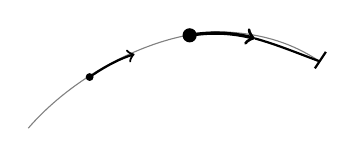
\begin{tikzpicture}[x=1cm,y=1cm]
\draw[gray,thin] (0,0) .. controls (0.65,0.75) and (1.75,1.27) .. (2.55,1.22) .. controls (3,1.19) and (3.35,1.08) .. (3.7,0.85);
\fill (0.78,0.65) circle (0.05);
\draw[thick,->] (0.78,0.65) .. controls (0.98,0.79) and (1.18,0.89) .. (1.35,0.94);
\fill (2.05,1.18) circle (0.09);
\draw[very thick,->] (2.05,1.18) .. controls (2.34,1.23) and (2.61,1.21) .. (2.88,1.14);
\draw[thick] (2.88,1.14) .. controls (3.17,1.06) and (3.48,0.93) .. (3.7,0.85);
\draw[thick] (3.64,0.76)--(3.78,0.97);
\end{tikzpicture}}

\uline{Th} On peut trouver, \inserted{de façon unique,} un syst. transitif d'iso entre les $\delta I$ $(I\in S)$ avec un quotient $\omega_S$, et un syst. transitif d'iso entre les $B_x$ $(x\in L)$, avec un quotient $\omega_L$, et une bijection $\omega_S\simeq\omega_L$ (soit $\underline{\omega}$ le quotient) -- donc un système d'iso $\underline{\omega}\simeq\delta I$, $\underline{\omega}\simeq B_x$, de façon que les conditions

\mspage{15}

\rotatebox{90}{\unsure{EXTRA STRONG}}
\rotatebox{90}{\unsure{EXTRA STRONG}}

\scanpage{17}
\mspage{14}

suivantes soient satisfaites

a) Si $I\supset J$, \inserted{\unsure{des segments}}, et si \deleted{$x_0\in\delta I$, \unsure{on}} \inserted{$\unsure{o_I|\sigma_I}$ est un des deux ordres canoniques sur $I$,} \deleted{alors $\delta I\simeq\delta J$ lui fait correspondre l'unique $y_0\in\delta J$ qui soit le plus petit élément de $J$ pour l'ordre} \inserted{alors $o_J:=o|J$ est un des deux ordres canoniques sur $J$, alors $\delta I\simeq\delta J$} associe au plus petit élément de $I$ le plus petit élément de $J$ (et idem pour le plus grand, par conséquent en \deleted{\unsure{en}} remplaçant $o$ par l'ordre opposé)

b) Si $I\in S$, et si $x_0\in\delta I$ est le plus petit élément pour \deleted{l'un des} \inserted{l'ordre} canonique $o$ sur $I$, alors \unsure{le} \deleted{\unsure{à}} $x_0\in\delta I$ correspond la branche en $\unsure{o|x}$ définie par $I$.

Il faut voir que la relation d'équivalence $R$ définie dans
\[
\coprod_{I\in S}\delta I\ \amalg\ \coprod_{x\in L}B_x
\]
par les relations élémentaires \deleted{$\unsure{R_a}\ \unsure{R_b^{\ast}}$} \inserted{\textcircled{a}, \textcircled{b}}
\[
(I,\underset{\substack{\rotatebox{-90}{$\in$}\\\delta I}}{x})
\underset{\substack{\deleted{\unsure{R_a}}\\\text{\textcircled{a}}}}{\sim}
(\unsure{I|J},y)
\quad\Longleftrightarrow\quad
J\subset I\text{ et }x\text{ et }y
\]
se correspondent par la \unsure{prescription} \unsure{a}
\[
(I,\underset{\substack{\rotatebox{-90}{$\in$}\\\delta I}}{x})
\underset{\text{\textcircled{b}}}{\sim}
\left(x,\underset{\substack{\text{branche}\\\text{en }x\text{ définie}\\\text{par }I}}{\underbrace{\beta(I,x)}}\right)
\]
admet exactement deux \uline{classes}, et que

\mspage{16}

\rotatebox{90}{\reflectbox{\unsure{EXTRA STRONG}}}
\rotatebox{90}{\reflectbox{\unsure{EXTRA STRONG}}}

\scanpage{18}
\mspage{15}

les deux éléments de $\delta I$, $I\in S$ (fixé) appartiennent à des classes distinctes \inserted{($\Longleftrightarrow$ idem pour les deux éléments des $B_x$, $x\in L$).}
\unsure{Je n'ai} pas la vérification ici. Si c'était faux, il faudrait le mettre en axiome. Sauf erreur, il doit être immédiat que \deleted{\unsure{il y a}} le nb de classes est $1$ ou $2$.

\deleted{On est orienté}

L'ens quotient $\underline{\omega}$ est l'ens des orientations de $\mathcal X$. \deleted{\unsure{On}} On a orienté $\mathcal X$ quand on a choisi $\omega\in\underline{\omega}$. Alors chaque $I$ a une origine, et pour chaque $x\in L$, on a un germe de segment \inserted{\uline{croissant}} issu de $x$ et d'origine $x$ (la \uline{branche sortante} de $x$).

Considérons alors la relation
\[
x<y\quad\overset{\mathrm{def}}{\Longleftrightarrow}\quad
\deleted{\unsure{x,y}}
\exists I\in S\text{ tel que }
\begin{array}{l}
x\in\operatorname{or}(I)\\
y\in\operatorname{ex}(I).
\end{array}
\]

Distinguons deux cas suivant que cette relation est transitive (\uline{cas linéaire}) ou non (cas circulaire).

I) Relation $x<y$ est transitive donc relation
\[
x\leq y\quad(\overset{\mathrm{def}}{\Longleftrightarrow}\ x=y\text{ ou }x<y)
\]
est un préordre,

\mspage{17}

\rotatebox{90}{\unsure{EXTRA STRONG}}
\rotatebox{90}{\unsure{EXTRA STRONG}}

\scanpage{19}
\mspage{16}

Je dis que c'est un \uline{ordre}, i.e. qu'on ne peut avoir $x<y$ et $y<x$ (en effet, on aurait $x<x$, ce qui est faux, car $x<y$ implique $x\unsure{=|\ne}y$). Les segments sont les $[x,y]$, pour $x<y$, et pour \unsure{tt} \inserted{tel} segment, son origine est $x$ (pour l'orientation choisie \inserted{son extrémité $y$}). Ainsi, la structure de modèle \inserted{connexe} orienté de $1$-forme régulier est connue quand on connaît la structure d'ordre. Celle-ci \deleted{est} satisfait les conditions

elle est \inserted{str.} filtrante croissante (i.e. $\forall x,y\in L$, $\exists z\in L$ t.q. $x,y<z$) et str. filtrante décroissante, elle est \inserted{str.} loc. filtrante décroissante et loc. filtrante \deleted{\unsure{str.}} croissante : (si $\deleted{\unsure{x<}}\inserted{x\leq}y,z$, $\exists u$ tel que $x\deleted{\unsure{\leq}}\inserted{<}u\deleted{\unsure{\leq}}\inserted{<}y,z$, et forme duale)

\margin{donc pas de plus grand ni de plus petit \unsure{élém$^{\mathrm t}$}}

\margin{implique que c'est divisible, i.e. si $x<y$, $\exists z$ avec $x<z<y$}

Prouvons p.ex. qu'elle est \unsure{str.} filtrante croissante.

\mspage{18}

\rotatebox{90}{\reflectbox{\unsure{EXTRA STRONG}}}
\rotatebox{90}{\reflectbox{\unsure{EXTRA STRONG}}}

\scanpage{20}
\mspage{17}

Soit $x,y\in L$. $\exists$ chaîne $x_0,x_1,\ldots x_n$ avec $x_0=x$, $x_n=y$ et $x_i,x_{i+1}\in I_i^\circ$. \deleted{\unsure{Quitte}} Quitte à rapetisser $I_i$, \deleted{\unsure{Posons}} Quitte

Posons $y_i=\operatorname{or}(I_i)$, alors on a
\[
x_i\unsure{>|\geq}y_i\unsure{<|\leq}x_{i+1}
\unsure{>|\geq}y_{i+1}\unsure{<|\leq}x_{i+2}
\]
donc $L$ en tant qu'ens ord. est connexe : On peut connecter deux éléments quelconques par une chaîne d'inégalités. On va raisonner sur la longueur. Si la chaîne est de longueur $\leq1$, donc $x\leq y$ il suffit de \deleted{prouver} \inserted{noter} qu'il existe $z$ avec $y<z$ (provenant du fait que $y$ régulier). Supposons que c'est prouvé pour $n-1$, \deleted{donc $\exists$} prouvons le pour $n$. \deleted{\unsure{x}} On suppose donc $\exists z$ avec
\[
x\underset{n-1}{\sim}z,\qquad z\underset{1}{\sim}y.
\]
Par hypothèse de récurrence, $\exists x'$ tel que \deleted{$\unsure{x<}$} $x,z<x'$. Si $z\geq y$ alors $x'>x,y$ on gagne. Si $z<y$ \unsure{le seul qui a}

\mspage{19}

\rotatebox{90}{\unsure{EXTRA STRONG}}
\rotatebox{90}{\unsure{EXTRA STRONG}}

\scanpage{21}
\mspage{18}

\diagram{\begin{tikzcd}[ampersand replacement=\&,row sep=small,column sep=small]
\& ? \arrow[dl,dashed,no head] \arrow[dr,dashed,no head] \& \&\\
y \arrow[dr,no head] \& \& x' \arrow[dl,no head] \arrow[dr,no head] \&\\
\& z \& \& x
\end{tikzcd}}

et il suffit de trouver $\unsure{t}$ tel que $t>\deleted{\unsure{y}}x',y$. Donc on est ramené à prouver ceci (filtration relative)

Si
\diagram{\begin{tikzcd}[ampersand replacement=\&,row sep=small,column sep=small]
\&v\\
u\arrow[ur,no head]\arrow[dr,no head]\&\\
\&w
\end{tikzcd}}
on peut compléter en
\diagram{\begin{tikzcd}[ampersand replacement=\&,row sep=small,column sep=small]
\&v\arrow[dr]\&\\
u\&\&t\\
\&w\arrow[ur]\&
\end{tikzcd}}

\deleted{\unsure{Il} manque visiblement \unsure{quelque chose}}

Mais on note qu'une relation d'ordre connexe qui est \uline{loc.} str. croissante et str. décroissante, et telle que pour \unsure{tt} élément $x$, $\exists x'_{\unsure{a}}<x<x''$, définit une structure de modèle de forme régulier connexe (on vérifie axiomes F1 à F5). Mais une telle structure n'est pas néc. filtrante croissante (\unsure{dito})

\mspage{20}

\rotatebox{90}{\reflectbox{\unsure{EXTRA STRONG}}}
\rotatebox{90}{\reflectbox{\unsure{EXTRA STRONG}}}

\scanpage{22}
\mspage{19}

\deleted{
Exemple : Considérons un nb réel irrationnel $r$, et considérons l'ens
\[
L=\underbrace{\mathbb Q\cap]-\infty,r]}_{L_1}
\amalg
\underbrace{(\mathbb Q\cap[r,+\infty])\times\varepsilon}_{L_2}
\]
où $\varepsilon$ est un ens \deleted{à deux} quelconque de card $\geq2$. On \deleted{peut} a donc
\diagram{\[\begin{array}{ccc@{\quad}l}
L&\overset{p}{\unsure{-|\longrightarrow}}&\mathbb Q&\text{(surjectif)}\\
L&\xrightarrow{q}&\varepsilon\amalg\{0\}&q(x)=0\text{ si }x\in L
\end{array}\]}
et si $x,y\in L$, on pose
\[
x<y\quad\Longleftrightarrow\quad px<py\quad\uline{\text{et}}
\]
}

\uline{Ex} Soit $L_0$ un ordonné \deleted{\unsure{str.}} \inserted{non vide} \deleted{filtrant croissant et filtrant} \deleted{str. filtrant} loc. str. filtrant croiss et décroissant, et telle que
\[
\exists x\in L_0,\ \exists x'<x<x'',
\]
et soit $L_i$ $(i\in I)$ une famille d'ens ordonnés satisfaisant les $=$s conditions. Soit
\[
L=L_0\amalg\coprod_iL_i.
\]
On met la relation d'ordre
\[
x<y\quad\unsure{\text{ssi}|\text{ssc}}\quad
\left|
\begin{array}{l}
\text{ou bien }x,y\text{ dans }\deleted{L_0}\inserted{\text{un }=L_0\text{ ou}}\\
\quad\text{un }L_i,\text{ et }x<y\text{ dans }\inserted{\text{cet}}L_i\\
\text{ou bien }x\in L_0,\ y\in L_i\quad(i\in I)
\end{array}
\right.
\]
Elle satisfait les $=$s conditions que $L_0,L_i$ mais n'est pas filtrante croissante !

\mspage{21}

\rotatebox{90}{\unsure{EXTRA STRONG}}
\rotatebox{90}{\unsure{EXTRA STRONG}}

\scanpage{23}
\mspage{20}

F6) Soient $I,J\in S$, \inserted{$x\in L$,} tels que $x\in\delta I$, $x\in\delta J$, et que $I,J$ définissent la $=$ branche i.e. $\exists y\in I^\circ\cap J^\circ$, \inserted{$y\ne x$,} tel que $I_{x,y}=J_{x,y}$. Alors $\exists K\in S$ tel que
\[
x\in\delta K,\ I^\circ\cup J^\circ\subset K^\circ.
\]

En d'autres termes, l'ens des \inserted{$I^\circ$,} $I\in S$ tels que $x\in\delta I$, et que $I$ appartienne à une branche donnée \inserted{en $x$,} est filtrant croissant pour l'inclusion.

\margin{\uline{NB} On n'exige pas que les autres extrémités \inserted{$\deleted{\unsure{\delta}}I,\deleted{\unsure{\delta}}J$} \unsure{de $I$} soient dans $K$. Mais \deleted{\unsure{il est clair}} que celles de ces extrémités qui sont régulières \unsure{soient} \deleted{\unsure{dans}} $K$ \unsure{Car conséquence de la propriété de dilatation|Car conséquence de la propriété d'extension} (Cor. 2 p. 7).}

Ou encore (en connexion avec F3)

Soient $I,J\in S$, $x\in L$ tels que $x\in\delta I\cap\delta J$. Alors

a) Pour qu'il existe $y\in I^\circ\cap J^\circ$ tel que
\[
I_{x,y}=J_{x,y},
\]
il f. et s. qu'il existe $K\in S$ tel que $x\in\delta K$, $I\cup J\subset K$

b) Si cette condition \unsure{n'est} vérifiée alors $\exists u\in I^\circ$, $v\in J^\circ$ tels que
\[
I_{x,u}\cap\unsure{I_{x,v}|J_{x,v}}=\{x\}.
\]

\mspage{22}

\rotatebox{90}{\reflectbox{\unsure{EXTRA STRONG}}}
\rotatebox{90}{\reflectbox{\unsure{EXTRA STRONG}}}

\scanpage{24}
\mspage{21}

(7 juin) \unsure{Une|Un} modèle de $1$-forme au sens précédent (ensemble de lieux $L$, avec ens de ``segments'' $S\subset\mathcal P(L)$, et $\forall I\in S$, un $\delta I\in\mathcal P_2(I)$, \deleted{\unsure{de}} de façon à satisfaire les conditions (F1) à (F6)) est appelé un \uline{réseau}.

Les lieux critiques \inserted{ou singuliers} ou de branchement sont appelés aussi \uline{noeuds} du réseau. Les comp. connexes de $L_r\setminus\underset{\text{noeuds}}{\underbrace{L_s}}$ sont \unsure{appelées} les \uuline{lignes} du réseau (de préférence à arêtes). Composantes connexes : les \uline{composantes} du réseau.

On parlera de l'\uline{ordre} ou de la \uline{multiplicité} d'un noeud (plus \unsure{général$^{\mathrm t}$|généralement}, d'un lieu du réseau -- elle est égale à $2$ en un lieu \uline{régulier}).

On dira qu'un \deleted{segment} \inserted{réseau} est \uline{divisible} \unsure{ssi} pour \unsure{tt} segment $I$, $I^\circ\ne\varnothing$.

On dira qu'il est \uline{réduit} si pour \unsure{tt} segment $I$, $I^\circ=\varnothing$ \inserted{i.e. $I=\delta I$ i.e. $\operatorname{card}I=2$}, ou encore si $L_r=\varnothing$, i.e. tous ses lieux sont des noeuds.

\mspage{23}

\rotatebox{90}{\unsure{EXTRA STRONG}}
\rotatebox{90}{\unsure{EXTRA STRONG}}

\scanpage{25}
\mspage{22}
La donnée d'une structure de réseau discret sur $L$ revient à celle d'une \deleted{structure} partie $S$ de $\mathcal P_2(L)$
[les axiomes F1) à F6) sont vides !]
donc une structure de \uline{graphe} réduit.

\begin{center}\rule{0.9cm}{0.7pt}\end{center}

[Je reviens à l'étude des réseaux réguliers \unsure{et} connexes (\inserted{et} non vides, i.e. 0-connexes)]

\deleted{Lemme}
On va étudier les cas de figure de deux segments ``consécutifs''

\margin{$\unsure{\mathcal R|R}$ quelconque avec $y$ \uline{régulier}}

\figure{\begin{tikzpicture}[x=1cm,y=1cm]
\draw (0,0)--(2.95,.13); \draw (3.25,.16)--(5.9,.35);
\draw (0,-.07)--(0,.07);
\fill (3.1,.15) circle(.035); \fill (5.9,.35) circle(.025);
\node[below] at (0,0) {$x$};
\node[below] at (3.1,.15) {$y$};
\node[below right] at (5.9,.35) {$z$};
\node[above] at (1.5,.08) {$I$};
\node[above] at (4.5,.24) {$J$};
\end{tikzpicture}}

avec \inserted{$y\in\delta I\cap\delta J$}, $\operatorname{br}_y(I)\ne\operatorname{br}_y(J)$, \inserted{$y\in L_r$}, Je distingue deux cas :

I) $I\cap J=\{y\}$ alors \deleted{\unsure{Si}} par axiome de recollement,
$\exists!K\in S$, $K\supset I\cup J$, $\delta K=\{x,z\}$,
et $I=K_{xy}$, $J=K_{yz}$. Situation bien comprise.

\deleted{II) $I\cap J\ne\{y\}$. \unsure{On distingue un} \inserted{Soit}

a) $x=z$

\deleted{\unsure{a)|ou} $I\cap J=\{y,x\}$}

\figure{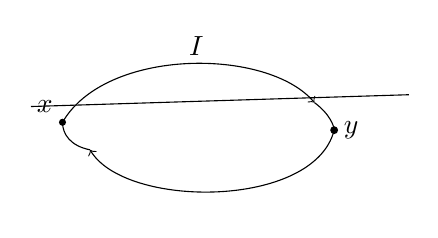
\begin{tikzpicture}[x=1cm,y=1cm]
\draw[->] (0,0) .. controls (.55,.95) and (2.6,.95) .. (3.2,.25);
\draw (3.2,.25) .. controls (3.4,.1) and (3.45,-.05) .. (3.45,-.1);
\draw[->] (3.45,-.1) .. controls (3.2,-1.1) and (.8,-1.1) .. (.35,-.35);
\draw (.35,-.35) .. controls (.1,-.3) and (0,-.15) .. (0,0);
\fill (0,0) circle(.045); \fill (3.45,-.1) circle(.05);
\node[above left] at (0,0) {$x$}; \node[right] at (3.45,-.1) {$y$};
\node[above] at (1.7,.72) {$I$};
\draw (-.4,.2)--(4.4,.35);
\end{tikzpicture}}

b) $I\cap J\ne\{y,x\}$ \unsure{si} $(x\ne y)$ \unsure{alors}

$\exists t\in I\cap J,\ t\ne y$.}
\mspage{24}

\rotatebox{90}{\reflectbox{\unsure{EXTRA STRONG}}}
\rotatebox{90}{\reflectbox{\unsure{EXTRA STRONG}}}

\scanpage{26}
\mspage{23}
II) $I\cap J\ne\{y\}$ \qquad Deux cas

\deleted{a) $\unsure{I\cap J=\{x,y\}}$}

\deleted{\figure{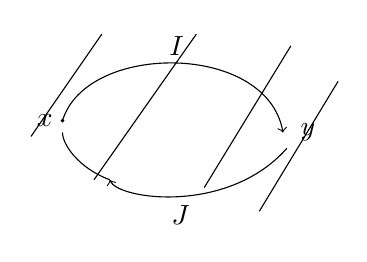
\begin{tikzpicture}[x=1cm,y=1cm]
\draw[->] (0,0) .. controls (.3,1) and (2.6,1) .. (2.8,-.15);
\draw[->] (2.85,-.35) .. controls (2.1,-1.2) and (.7,-1) .. (.6,-.75);
\draw (.6,-.75) .. controls (.2,-.6) and (0,-.3) .. (0,-.15);
\fill (0,0) circle(.025);
\node[left] at (0,0) {$x$}; \node[right] at (2.9,-.15) {$y$};
\node[above] at (1.45,.7) {$I$}; \node[below] at (1.5,-.95) {$J$};
\draw (-.4,-.2)--(.5,1.1); \draw (.4,-.75)--(1.7,1.1);
\draw (1.8,-.85)--(2.9,.95); \draw (2.5,-1.15)--(3.5,.5);
\end{tikzpicture}}}

\deleted{b) $x\ne y$}
Soit $w\in I\cap J$, $w\ne y$
et considérons
\[
\begin{array}{c}
\uline{J_{y,w}}\\[-.4ex]
\rotatebox{-90}{$\in$}\\[-.4ex]
S
\end{array}
\subset J,\quad \uline{I_{w,y}}
\]

\margin{\figure{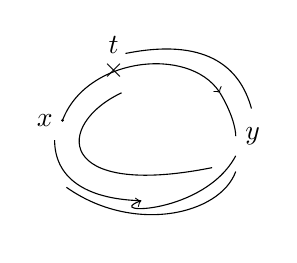
\begin{tikzpicture}[x=1cm,y=1cm]
\draw[->] (0,0) .. controls (.3,.8) and (1.6,.95) .. (2,.35);
\draw (2,.35) .. controls (2.15,.1) and (2.2,-.1) .. (2.2,-.2);
\draw[->] (2.2,-.45) .. controls (1.8,-1.2) and (.5,-1.2) .. (1,-1.02);
\draw (1,-1.02) .. controls (.25,-1) and (-.1,-.7) .. (-.1,-.25);
\draw (.8,.85) .. controls (1.8,1.05) and (2.25,.7) .. (2.4,.15);
\draw (.75,.35) .. controls (-.1,-.05) and (-.1,-1) .. (1.9,-.6);
\draw (.05,-.85) .. controls (.9,-1.45) and (2,-1.2) .. (2.2,-.65);
\fill (0,0) circle(.02); \node[left] at (0,0) {$x$};
\node[right] at (2.2,-.2) {$y$};
\node at (.65,.63) {$\times$}; \node[above] at (.65,.72) {$t$};
\end{tikzpicture}}}

\figure{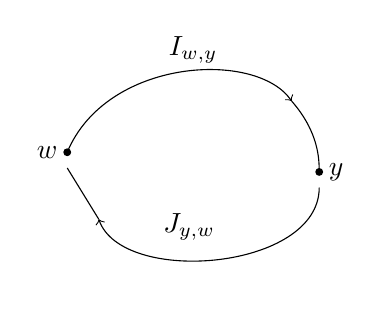
\begin{tikzpicture}[x=1cm,y=1cm]
\draw[->] (0,0) .. controls (.5,1.2) and (2.4,1.3) .. (2.85,.65);
\draw (2.85,.65) .. controls (3.2,.25) and (3.2,-.1) .. (3.2,-.25);
\draw[->] (3.2,-.45) .. controls (3.2,-1.5) and (.7,-1.7) .. (.4,-.85);
\draw (.4,-.85)--(0,-.2);
\fill (0,0) circle(.05); \fill (3.2,-.25) circle(.05);
\node[left] at (0,0) {$w$}; \node[right] at (3.2,-.25) {$y$};
\node[above] at (1.6,1) {$I_{w,y}$};
\node at (1.55,-.95) {$J_{y,w}$};
\end{tikzpicture}}

\margin{\uline{NB} $w$ régulier \uline{sauf} si \deleted{$w\in\{x,z\}$}
$w=x=z$ \deleted{\unsure{et}} i.e.
si on
\figure{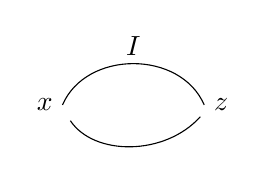
\begin{tikzpicture}[x=1cm,y=1cm]
\draw (0,0) .. controls (.3,.7) and (1.5,.7) .. (1.8,0);
\draw (.1,-.2) .. controls (.4,-.65) and (1.3,-.65) .. (1.75,-.15);
\node[left] at (0,0) {$x$}; \node[right] at (1.8,0) {$z$};
\node[above] at (.9,.5) {$I$};
\end{tikzpicture}}}

\deleted{Je dis que $I_{w,y}\cap$}

Je vais donc étudier d'abord la situation

\figure{\begin{tikzpicture}[x=1cm,y=1cm]
\draw[->] (0,0) .. controls (.2,1) and (1.3,1.4) .. (2.1,1.05);
\draw (2.1,1.05) .. controls (2.6,.8) and (2.9,.3) .. (3,0);
\draw[->] (3,-.25) .. controls (3,-1.8) and (.4,-1.7) .. (.1,-.4);
\draw[dashed] (1,1.08)--(1,-1.35);
\draw (0,0) circle(.035); \fill (3,0) circle(.05);
\fill (1,1.08) circle(.04); \fill (1,-1.35) circle(.04);
\node[left] at (0,0) {$x$}; \node[right] at (3,0) {$y$};
\node[above] at (1,1.08) {$t$}; \node[below] at (1,-1.35) {$t$};
\node[above] at (1.65,1.3) {$I$}; \node at (1.7,-1.05) {$J$};
\end{tikzpicture}}

\margin{$\operatorname{br}_y I\ne\operatorname{br}_y J$

\uline{NB} On ne va pas exiger $y$ régulier}

\deleted{$I\cap J\unsure{=}$}
\[
\delta I=\delta J,\quad I\cap J=?
\]
Je dis que $\operatorname{br}_x(I)\ne\operatorname{br}_x(J)$. Sinon,
en vertu de l'axiome F6, existerait $K\in S$, tel que :
$x\in\delta K$, et $I=K_{x,y}$, $J=K_{xy}$
donc $I=J$, donc $\operatorname{br}_y(I)=\operatorname{br}_y J$, absurde.

Je dis que $I\cap J=\{x,y\}$. Si on avait
$t\in I\cap J$, $t\notin\{x,y\}$, donc $t\in I^\circ\cap J^\circ$,
\unsure{en appliquant|on appliquerait} ce qui précède à $I_{x,t}$, $J_{x,t}$
\mspage{25}

\rotatebox{90}{\unsure{EXTRA STRONG}}
\rotatebox{90}{\unsure{EXTRA STRONG}}

\scanpage{27}
\mspage{\unsure{24|29}}
(car
$\begin{array}{ccc}
\operatorname{br}_x I_{x,t}&\ne&\operatorname{br}_x J_{x,t}\\
\unsure{\Vert|\text{''}}&&\unsure{\Vert|\text{''}}\\
\operatorname{br}_x I&&\operatorname{br}_x(J)
\end{array}$
) on aurait
$\operatorname{br}_t I_{x,t}\ne\operatorname{br}_t J_{x,t}$, donc en vertu de l'axiome des \deleted{branches} $p^{ts}$ réguliers (F5) on aurait $\operatorname{br}_t$

\rotatebox{90}{\reflectbox{\unsure{EXTRA STRONG}}}
\rotatebox{90}{\reflectbox{\unsure{EXTRA STRONG}}}
\mspage{26}

\cotefile{156-2}
\scanpage{1}
\figure{
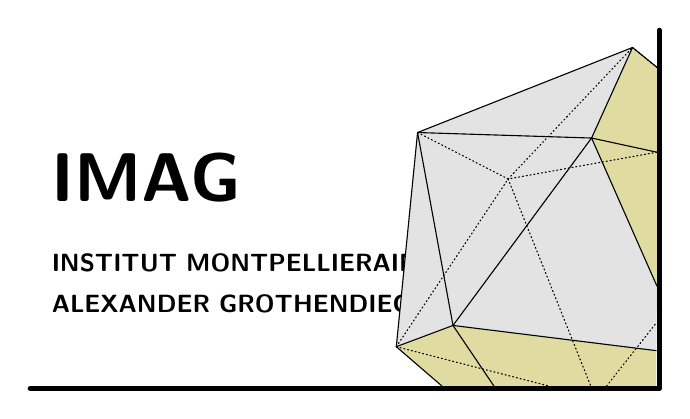
\begin{tikzpicture}[x=1cm,y=1cm,line join=round,line cap=round]
\node[anchor=west,font=\sffamily\bfseries\fontsize{40}{44}\selectfont] at (-4.5,2.65) {IMAG};
\node[anchor=west,font=\sffamily\bfseries\fontsize{9}{11}\selectfont] at (-4.5,1.56) {INSTITUT MONTPELLIERAIN};
\node[anchor=west,font=\sffamily\bfseries\fontsize{9}{11}\selectfont] at (-4.5,1.05) {ALEXANDER GROTHENDIECK};
\coordinate (A) at (0,0.50);
\coordinate (B) at (0.27,3.22);
\coordinate (C) at (3.00,4.30);
\coordinate (D) at (3.32,4.04);
\coordinate (E) at (3.31,2.97);
\coordinate (F) at (3.31,1.27);
\coordinate (G) at (3.30,0.00);
\coordinate (H) at (0.58,0.00);
\coordinate (I) at (0.72,0.77);
\coordinate (J) at (2.48,3.15);
\coordinate (K) at (1.42,2.63);
\fill[gray!22] (A)--(B)--(C)--(J)--(F)--(G)--(H)--cycle;
\fill[olive!28] (C)--(D)--(E)--(J)--cycle;
\fill[olive!28] (J)--(E)--(F)--cycle;
\fill[olive!28] (A)--(I)--(3.30,0.45)--(G)--(H)--cycle;
\draw (A)--(B)--(C)--(D);
\draw (C)--(J)--(F);
\draw (B)--(J)--(E);
\draw (B)--(I)--(1.24,0);
\draw (A)--(I)--(J);
\draw (I)--(3.30,0.45);
\draw[densely dotted] (A)--(K)--(C);
\draw[densely dotted] (B)--(K)--(E);
\draw[densely dotted] (K)--(2.47,0);
\draw[densely dotted] (A)--(1.94,0);
\draw[densely dotted] (2.67,0)--(3.30,0.80);
\draw[densely dotted] (C)--(D);
\draw (A)--(H);
\draw[line width=1.8pt] (-4.65,-0.03)--(3.34,-0.03)--(3.34,4.52);
\end{tikzpicture}
}

\scanpage{2}
\mspage{1}
Réalisations topologiques des réseaux \hfill (Juin 86)

\margin{\unsure{CF II|Ch II}}

1. Ficelle topologique. (6 Juin)

Soit $X$ espace top., $A\subset X$ partie fermée \inserted{non vide} de $X$.
\deleted{\unsure{Soit}} $X/A$ l'espace déduit de $X$ en contractant $A$ en un pt,
\inserted{$a$ le $p^t$ déduit de $A$ par contraction.}
Si $X'$ est une partie de $X$ contenant $A$, alors $X'/A\hookrightarrow X/A$ identifie $X'/A$ à un sous-espace top. de $X$
[les fermés de $X'/A$ s'identifient aux fermés \inserted{$Y'$} \deleted{\unsure{$Y$}} de $X'$ qui ou bien contiennent $A$, ou bien ne le rencontrent pas (i.e. tels que $Y'\cap A\in\{\varnothing,A\}$), et ce sont les traces sur $X'$ des fermés $Y$ de $X$ qui ont ces \unsure{$=$s|$\Longrightarrow$} propriétés, lesquels correspondent \inserted{d'ailleurs} aux fermés de $X/A$ \ldots]

On dit que $A$ est \uline{régulièrement immergé} dans $X$
si $\exists$ voisinage \deleted{\unsure{$V$}} conique de $a$ dans $X/A$
i.e. voisinage \inserted{\uline{fermé}}
$V\overset{h}{\simeq}\operatorname{\text{Cône}}(\unsure{B|S})$
$\unsure{B|S}$ espace topologique compact, $h(a)=o$.
(centre du cône),
\inserted{et $V^\circ=V\setminus B$ ouvert dans $X/A$.}
\deleted{Sur $V$} Alors \deleted{\unsure{le}} sur $V$ il y a (via $h$) une structure conique et en part. considérons les
\[
tV=V_t\qquad 0\le t\le1
\]
qui sont, pour $t\in]0,1]$, homéom. à $V$, et forment

\margin{\unsure{Souvent dit} ``\unsure{saturé}'' \deleted{\unsure{dans}} \unsure{d'après}
\deleted{\unsure{NB} \unsure{d'usage} $\unsure{\partial V|V^\circ}$ \illegible{2}}}

\margin{\uline{NB} $\dot V=B$\quad $\dot V_t=B_t$}
\mspage{1}

\rotatebox{90}{\unsure{EXTRA STRONG}}
\rotatebox{90}{\unsure{EXTRA STRONG}}

\scanpage{3}
\mspage{2}
un système fond. de voisinages de $a$ dans $X/A$.
Les $V_t^\circ=tV^\circ$, où $V^\circ=V\setminus B$,
forment un syst. fond. de voisinages.

\margin{$V_t=V_t^\circ\amalg B_t$}

Les images inverses $W_t$ de $V_t$ dans $X$ font un syst. fond. de voisinages de $A$ dans $X$.
\deleted{\unsure{Lemme}} Pour tout tel $W_t$, \deleted{\unsure{a}} $B_t$
\inserted{\unsure{noté} $=\dot W_t$ \unsure{aussi|d'où}} est
un fermé de $X$, et posant \deleted{\unsure{le}}
\[
W'_t=X-V_t,
\]
\deleted{On a}
\[
X\setminus\underbrace{B_t}_{\substack{\text{bord}\\\text{de }W_t}}
=
\underbrace{W_t^\circ}_{\substack{\text{int de}\\W_t}}
\amalg
\underbrace{W'_t}_{\substack{\text{ext de}\\W_t}}
\qquad\text{somme topologique}
\]

\uline{NB} \textcircled{1} L'hyp. faite sur $A\subset X$ est \uline{locale}
i.e. \deleted{Soit} $X'$ voisinage de $A$ dans $X$,
elle est vraie pour $(A,X)$ ssi elle est vraie pour $(A,X')$.

\textcircled{2} [Elle a un sens aussi pour $A=\varnothing$,
$X/\varnothing=\{a\}\amalg X$ on a alors $B=\varnothing$]

\textcircled{3} Vraie pour $A$ \inserted{sous-espace} \uline{modéré} compact dans esp. modéré $X$
(p.ex. \deleted{\unsure{espace}} triangulé et sous-ens. \unsure{compact poly.})

\margin{\textcircled{4}
$A$ est ouvert $\Longleftrightarrow$ $a$ est pt isolé
\inserted{$X/A$}
$\Longleftrightarrow B=\varnothing$}

\uline{Définition} Une \uline{ficelle topologique}
est un couple $(X,\{A,B\})$ formé d'un espace topologique $X$, et d'une paire
$\{A,B\}\in\mathcal P_2(\mathcal P(\unsure{A|X}))$ de parties de $X$.

\rotatebox{90}{\reflectbox{\unsure{EXTRA STRONG}}}
\rotatebox{90}{\reflectbox{\unsure{EXTRA STRONG}}}
\mspage{2}

\scanpage{4}
\mspage{3}
satisfaisant les conditions

Fic a) $A$ et $B$ sont \deleted{régulièrement immergés dans $X$.}
\inserted{fermés, \unsure{non-ouverts|non ouverts} (donc non vides)}
[Donc le $p^t$ $a$ de $X/A$ et le pt $b$ de $X/B$ sont non isolés
i.e. $S_A\ne\varnothing$, $S_B\ne\varnothing$

Fic b) \deleted{$\unsure{X}$} $A\cap B=\varnothing$

c) $(X\setminus A)/B$ et $(X\setminus B)/A$ sont connexes

Fic d) $A$ et $B$ sont régulièrement immergés.

\margin{Mais $X\ne A\cup B$ car $A,B$ non ouverts donc $U=X\setminus(A\cup B)$ est non vide}

\deleted{La condition c) peut se formuler}

On va donner \deleted{\unsure{des}} \inserted{une} variante de c) :

\deleted{ainsi}
c') \inserted{Pour} Toute composante connexe \inserted{$U_i$} de $U=X\setminus(A\cup B)$,
\inserted{$\overline{U_i}$} rencontre $B$ et rencontre $A$

On a
\[
c'\Longrightarrow c,
\]
et l'inverse est vrai si $U$ n'a qu'un $\unsure{n^\circ|n^{bre}}$ fini de composantes connexes
(cas $X,A,B$ modérés, notamment)

\margin{\uline{conditions} des ficelles réduites :
a) $a$ et $b$ \deleted{pts fermés} \inserted{non isolés}
b) $a\ne b$
c) $X\setminus\{a\}$ et $X\setminus\{b\}$ connexes
d) $a$ et $b$ ont des vois. coniques}

\margin{\uline{NB} Si $(X,\{A,B\})$ est une ficelle et $C\subset U=X\setminus(A\cup B)$ fermé dans $X$, alors $(X/C,\{\unsure{AB|A,B}\})$ est une ficelle.}

\margin{$c'\Downarrow c$}

$A$ et $B$ sont les \uline{bouts} \inserted{\uline{= extrémités}} de la ficelle $(X,\{A,B\})$.
La ficelle est réduite si $A,B$ sont réduits à un pt.
\inserted{$a,b$. On dit que $(X,\{a,b\})$ est une ficelle.}

Soit $X'$ déduit de $X$ en contractant $A,B$ en des pts,
$A\unsure{\mapstochar\relbar|\mapsto}a$ et $B\unsure{\mapstochar\relbar|\mapsto}b$,
$a,b\in X'$.

\margin{$X'={}_A\backslash X/B$}

Alors $(X,\{A,B\})$ est une ficelle ssi
$\{X',\deleted{\unsure{\{a}}\{a,b\}\}$ est une ficelle.

\margin{\uline{NB} Ficelle réduite est \uline{connexe}}

\rotatebox{90}{\reflectbox{\unsure{EXTRA STRONG}}}
\rotatebox{90}{\reflectbox{\unsure{EXTRA STRONG}}}
\mspage{3}

\scanpage{5}
\mspage{4}
\uline{Lieu} sur une ficelle $(X,\{A,B\})$ ;
c'est une partie \inserted{fermée} $C\subset X$ telle que
l'on ait les propriétés : ou bien $C\in\{A,B\}$,
ou bien les propriétés suivantes sont satisfaites.

\margin{\uline{NB} \inserted{Pour} une ficelle réduite $(X',\{a,b\})$,
$X'$ est connexe, ainsi que $X'\setminus\{b\}$ et $X'\setminus\{a\}$
(\unsure{ouverts de|autour de} $X'$) mais pas néc. $X'\setminus\{a,b\}$.
\figure{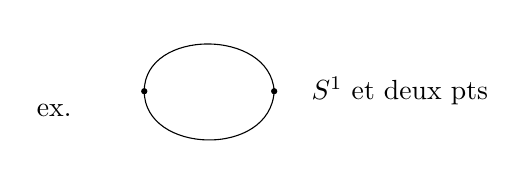
\begin{tikzpicture}[x=1cm,y=1cm]
\draw (0,0) .. controls (0,.8) and (1.6,.8) .. (1.65,0)
.. controls (1.6,-.85) and (0,-.8) .. (0,0);
\fill (0,0) circle(.04); \fill (1.65,0) circle(.04);
\node[left] at (-.8,-.25) {ex.};
\node[right] at (2,0) {$S^1$ et deux pts};
\end{tikzpicture}}}

\deleted{Li a) $C$ fermée, et $C\in\{A,B\}$ ou $C\subset U$
\inserted{$X\setminus(A\cup B)$}}

\deleted{\unsure{b)}
($C$ est l'une des extrémités, ou n'en rencontre aucune)}

Li a) $\exists$ décomposition de $X\setminus C$ en somme \inserted{\unsure{top.}} de deux sous-espaces
\[
\unsure{\deleted{U}\inserted{X}|\deleted{X}\inserted{U}}_{A,C},\quad \unsure{\deleted{U}\inserted{X}|\deleted{X}\inserted{U}}_{B,C}
\]
\[
A\subset\unsure{\deleted{U}\inserted{X}|\deleted{X}\inserted{U}}_{A,C}
\qquad
B\subset\unsure{\deleted{U}\inserted{X}|\deleted{X}\inserted{U}}_{B,C}
\]
et
\[
\unsure{\deleted{U}\inserted{X}|\deleted{X}\inserted{U}}_{A,C}/A
\quad\text{et}\quad
\unsure{\deleted{U}\inserted{X}|\deleted{X}\inserted{U}}_{B,C}/B
\]
connexes
[et ceci détermine $X_{A,C}$, $X_{B,C}$ de façon unique,
comme images inverses des comp. conn. de
$\underset{\inserted{\begin{array}{c}\unsure{\Vert|\text{''}}\\{}_A\backslash X/B\end{array}}}{X'}\setminus C$
qui contient

\margin{i.e. $X'\setminus C$ a deux comp. connexes, dont l'une contient $a$, l'autre contient $b$}

\margin{\uline{NB} \unsure{Quand} $A,B$ connexes,
$U_{A,C}$, $U_{B,C}$ \deleted{\unsure{sont}} sont connexes
donc \unsure{les c.c.} de $X\setminus C$}

\rotatebox{90}{\reflectbox{\unsure{EXTRA STRONG}}}
\rotatebox{90}{\reflectbox{\unsure{EXTRA STRONG}}}
\mspage{4}

\scanpage{6}
\mspage{5}
\uline{NB} Soit
\[
X_{A,C}=\overline{U_{A,C}}\cup C,\quad
X_{B,C}=\overline{U_{B,C}}\cup C
\]
Je dis que $(X_{A,C},\{A,C\})$ satisfait les conditions a) b) c) des ficelles
(donc il en sera de $=$ de $(X_{B,C},\{B,C\})$).

Pour le voir, on est ramené au cas $A,B,C$ réduits à des pts, $a,b,c$.
Il faut prouver que

a) \deleted{$\unsure{a}$} $c$ n'est pas isolé dans $X_{a,c}$,
\inserted{$a$ n'est pas isolé dans $X_{a,c}$ puisqu'il ne l'est pas dans $X$ et $X_{a,c}$ en est un vois. \unsure{de $a$}.}
\unsure{sinon} \deleted{On} aurait $U_{ac}$ ouvert et fermé dans $X$,
$X$ \inserted{serait} non connexe, absurde.

b) $X_{a,c}\setminus\{c\}$ est connexe par hyp.
Je dis que $X_{a,c}\setminus\{a\}$ est connexe.
Sinon, \deleted{\unsure{avait}} $\exists$ partie $V$ de $X_{ac}\setminus\{\unsure{a}\}$ qui soit ouverte et fermée dans $X_{ac}\setminus\{a\}$,
non vide, et ne contient pas $c$.
Donc elle serait aussi \deleted{ouverte} (fermée et) \uline{ouverte}
dans $X\setminus\{a\}$, sans \deleted{\unsure{contenir}} être tout,
$X\setminus\{c\}$ ne serait pas connexe, absurde.

Pour que $(X_{A,C},\inserted{\{A,C\}})$ soit une ficelle,
il manque encore l'\unsure{hypothèse} d) d'immersion locale.

\rotatebox{90}{\reflectbox{\unsure{EXTRA STRONG}}}
\rotatebox{90}{\reflectbox{\unsure{EXTRA STRONG}}}
\mspage{5}

\scanpage{7}
\uline{Lemme} Soit $Z$ un espace, $Z'$ et $Z''$ deux parties fermées, telles que
$Z'\cap Z''=\{c\}$.
Pour que $c$ ait un voisinage conique dans $Z$, il f. et s. qu'il ait vois. conique dans $Z'$ et $Z''$.

Il est donc suffisant, pour avoir \deleted{\unsure{une}} décomposition de la ficelle en deux, d'imposer la condition

Li c) \uline{$C$ est régulièrement immergé dans $U$.}

\uline{Exemple} Pour $t$ assez petit, les $\unsure{\dot U|\dot V}_{A,t}=S_{A,t}$ sont des \deleted{\unsure{les}} lieux de la ficelle.

\margin{\uline{NB} Pour que $C$ partie fermée de $X$,
$\subset U=X\setminus(A\cup B)$, soit un lieu,
il f. et s. que \deleted{\unsure{dans}} $C\ne\varnothing$ et que
$\unsure{(X/_{A,B,C},\{a,b\}),\{c\}}$ soit un lieu.}

\margin{\deleted{Si $D$ est une partie fermée}
Si $D$ est une partie fermée de $X$ telle que \deleted{$\unsure{D\subset X\setminus(A\cup B\cup C)}$}
$D\subset\unsure{U|X}_{A,C}$ \uline{ou} $D\subset U_{B,C}$
(p.ex. \unsure{$D$ connexe}) alors
$C$ est \unsure{encore} un lieu de la ficelle
$\unsure{(X/D,\{A,B\})}$.}

\uline{Lieux disjoints.}
Soit $F=(X,\{A,B\})$ une ficelle, $\mathcal L(F)$ l'ens. de ses lieux.
Je vais définir une relation symétrique

``$C$ et $D$ sont disjoints''. \qquad $(\Longrightarrow(C\ne D))$

Quand $C$ \uline{ou} $D$ sont $\in\{A,B\}$, alors
``disjoints'' signifie simplement \uline{distinct}
($\Longleftrightarrow$ disjoints au sens ens., $C\cap D=\varnothing$).

\margin{\unsure{ou bien} $\{C,D\}=\{A,B\}$,
\unsure{ou bien l'un des deux} $C,D$ $\in\{A,B\}$, l'autre}

\rotatebox{90}{\reflectbox{\unsure{EXTRA STRONG}}}
\rotatebox{90}{\reflectbox{\unsure{EXTRA STRONG}}}
\mspage{6}

\scanpage{8}
\mspage{7}
\uline{Découpage} d'une ficelle \inserted{$F=(X,\{A,B\})$}
par un lieu $C$ distinct des extrémités : ficelles $F_{A,C}$, $F_{B,C}$.
Tout lieu d'une des ficelles composantes est un lieu de $F$.

\deleted{\unsure{Ficelle}}
\margin{(Pour \uline{mémoire})
\uline{Équiv. de Catégories}
a) Ficelles avec un lieu intérieur.
b) Paires de ficelles, avec un homéo entre un bout de l'une, un bout de l'autre.
$\Downarrow$}

\deleted{c'est un lieu \unsure{de $F$}}
\deleted{Soient}

\begin{tabular}{|p{0.9\linewidth}}
\uline{Lemme.} Soient $C$ et $D$ deux lieux de $F$, distincts des extrémités, avec \inserted{$C\ne D$}.
Alors $D$ est un lieu de $F_{B,C}$ ssi $C$ est un lieu de $F_{A,D}$.
(Donc, en échangeant les rôles de $A$ et $B$, \deleted{D est un} \inserted{ou de} $C$ et $D$,
$D$ est un lieu de $F_{A,C}$ ssi $C$ est un lieu de $F_{B,D}$.)
\end{tabular}

\margin{\diagram{\begin{tikzcd}[ampersand replacement=\&,column sep=small]
A \arrow[rr,no head,to path={-- ([yshift=-5mm]\tikztostart.south) -- ([yshift=-5mm]\tikztotarget.south) -- (\tikztotarget.south)}]
\& C \arrow[rr,no head,to path={-- ([yshift=5mm]\tikztostart.north) -- ([yshift=5mm]\tikztotarget.north) -- (\tikztotarget.north)}] \& D \& B
\end{tikzcd}}}

Démonstration : Il suffit de prouver $\Longrightarrow$
\deleted{\unsure{quand}.}
(l'autre implication en résulte, en \deleted{permutant} \inserted{éch.} $A$ et $B$, $C$, et $D$)
OPS $A,B,C,D$ réduits à des points.
On a par hypo \deleted{($c$ lieu de $X$)}
\[
\underset{\substack{\vert\\\text{car }c\text{ lieu}\\\text{de }X}}{X}
=
X_{a,c}\amalg_c
\underbrace{X_{c,b}}_{\substack{\unsure{\Vert|\text{''}}\,\text{déf}\\X_{b,c}}}
\qquad\text{et}\qquad
\underset{\substack{\vert\\\text{car }d\text{ lieu}\\\text{de }X_{c,b}}}{X_{c,b}}
=
X_{c,d}\amalg_d
\underbrace{X_{d,b}}_{\substack{\unsure{\Vert|\text{''}}\,\text{déf}\\X_{b,d}}}
\]
donc
\[
X=\underbrace{X_{a,c}\amalg_c X_{c,d}}_{X_{a,d}}\amalg_d X_{d,b}
\]

\rotatebox{90}{\reflectbox{\unsure{EXTRA STRONG}}}
\rotatebox{90}{\reflectbox{\unsure{EXTRA STRONG}}}
\mspage{7}

\scanpage{9}
\mspage{8}

\uline{Lieux disjoints} \inserted{$C,D$} sur une ficelle \inserted{(relation symétrique)}:

\deleted{ou bien $C$}
Si $C$ ou $D$ est une extrémité, \uline{disjoint} signifie que $C\ne D$. Si ni $C$ ni $D$ n'est une extrémité, alors disjoint signifie que
\deleted{\unsure{Si}} $C\ne D$, \uline{et} que $D$ est un lieu de $F_{A,C}$ ou de $F_{B,C}$ ($\Rightarrow C$ est un lieu de $F_{B,D}$ ou de $F_{A,D}$).

\uline{Ficelle orientée} Ficelle avec extrémité fixée (``origine).

\deleted{\unsure{A}} La catégorie des ficelles \inserted{orientées} munies de deux lieux internes \uline{disjoints}, est équivalente à celle des \deleted{systèmes} \deleted{triplets}\inserted{quintuplets} $(F_1,\unsure{F_1|F_2},F_3,h_{21},h_{32})$, où $F_1,F_2,F_3$ sont des ficelles orientées,
\[
h_{21}:\operatorname{ex}(F_1)\simeq\unsure{\operatorname{or}}(F_2),\quad
h_{32}:\operatorname{ex}(F_2)\simeq\operatorname{or}(F_3).
\]

$F=(X,(A,B))$ ficelle ordonnée. Soit $C$ un lieu, on pose $\unsure{\mathcal F_C|F_C}={}\text{ens des lieux de }F_{A,C}$.
\margin{si $C\ne A,B$; $=\{A\}$ si $C=A$, $=\unsure{F|\mathcal L}$ si $C=B$.}
On écrit $C\le D$ ssi $F_C\subset F_D$. Cela signifie aussi que $C\in F_D$.

\rotatebox{90}{\reflectbox{\unsure{EXTRA STRONG}}}
\rotatebox{90}{\reflectbox{\unsure{EXTRA STRONG}}}

\scanpage{10}
\mspage{9}

Les lieux d'une ficelle \inserted{orientée} forment un ens ordonné $\mathcal L$. Il satisfait les conditions suivantes
\margin{\unsure{Attention|Autre déf.} $X_{A,C}\subset X_{A,D}$ (et \deleted{$\unsure{C\le D}$} $\Leftrightarrow$ $\unsure{=}$ $X_{A,C}=X_{A,D}$) \unsure{n'implique} \uline{pas} que $C\le D$!}

a) $\exists$ plus petit et plus grand élément \inserted{$\alpha$ et $\beta$} distincts

b) $\forall x\in\mathcal L$, \deleted{\unsure{si} \unsure{$y,z$ sont des $y$}} \inserted{$x\ne\beta$, l'ens des élts $>x$ est} filtrant décroissant;

b') $\forall x\in\mathcal L$, $x\ne\alpha$, l'ens des \unsure{élts|éléments} $<x$ est filtrant croissant

c) Si $x<y$, $\exists z$ avec $x<z<y$ (divisibilité)

\uline{NB} \textcircled{1} Deux lieux \inserted{$x,y$} sont \uline{disjoints}, \deleted{ils} ssi $x<y$ ou $y<x$. Ils définissent une ficelle $F_{x,y}=F_{y,x}$.

\margin{\textcircled{2} Si on \unsure{prend l'or.} \unsure{opposée}, \deleted{\unsure{défini}} \unsure{ordre opposé}.}

\unsure{Considérons maintenant $n$} lieux intermédiaires, \uline{mutuellement disjoints} (i.e. \unsure{font|forment} une partie totalement ordonnée). La catégorie des syst. formés d'une ficelle orient. \inserted{$F$} et de $n$ tels lieux \inserted{$x_1\cdots x_n$} est équivalente à celle des systèmes $(F_1,\ldots,F_{n+1},h_{21},h_{32},\ldots,h_{n+1,n})$ de $n+1$ ficelles orientées, et de $n$ homeo. de raccordement.

\rotatebox{90}{\reflectbox{\unsure{EXTRA STRONG}}}
\rotatebox{90}{\reflectbox{\unsure{EXTRA STRONG}}}
\mspage{9}

\scanpage{11}
\mspage{10}

\uline{Conditions particulières sur les lieux.}

\uline{NB} Pour qu'un espace compact triangulable admette une structure de ficelle, il f. et s. qu'il soit connexe, et non réduit à un point. C'est gros! Il y a alors $=$ une structure de ficelle réduite. [NB. Si $X$ est un segment cette str. est unique. C'est le seul cas d'exception!]

\margin{\uline{NB} les seules \deleted{structures}\unsure{de|\deleted{de}}\inserted{ficelles} sur $[0,1]$ sont données par $\{A,B\}$ où $A=[0,\alpha]$, $B=[\beta,1]$ avec $0\le\alpha<\unsure{\beta'|\beta}\le1$. \deleted{\unsure{NB}}}

On peut considérer relation d'équivalence entre structures de ficelles \deleted{sur $X$} (resp. ficelles orientées) sur $X$: \deleted{\unsure{p}} celle engendrée par la relation d'ordre (cas orienté)
\deleted{ou \unsure{$(A\subset A'\ \text{ou}\ A\subset B')$ et $(B\subset A'\ \unsure{,|\text{ou}}\ B\subset B')$}}
\[
A\subset A'\quad\text{et}\quad B\subset B'.
\]

\margin{Il est \unsure{raisonnable} de supposer les extrémités $A,B$ (\unsure{de même} $A',B'$) connexes voire, \unsure{contractiles}.}
\deleted{Oui}
\deleted{\uline{NB} Si $(X,\{A,B\})$ est une ficelle, et si $A',B'$ sont des fermés régulièrement immergés tels que $A\subset A'$, $B\subset B'$, $A'\cap B'=\varnothing$, alors $(X,\{A',B'\})$ est une ficelle.}
\margin{Faux $\longrightarrow$ idiot!}
\margin{(\unsure{Connexité})}

\deleted{donc}\inserted{soupçonne} que deux structures de ficelle orientée sur un $X$ triangulable sont toujours équivalentes.
\margin{Faux déjà dans le cas du segment!}

\rotatebox{90}{\reflectbox{\unsure{EXTRA STRONG}}}
\rotatebox{90}{\reflectbox{\unsure{EXTRA STRONG}}}
\mspage{10}

\scanpage{12}
\mspage{11}

\deleted{\unsure{Considérons}}
On peut imposer des conditions à $A,B$, comme d'être connexes, voire, contractiles, voire $=$, homéom. à un espace donné, et itou pour les lieux, \inserted{de façon à travailler sur un sous-ens $\mathcal L_P$, $P$ propriété \unsure{intrinsèque}}.

Pour que les conditions plus haut sur l'ens \uline{ordonné} $\mathcal L$ soient encore vraies pour $\mathcal L_P$, il est bon de \deleted{\unsure{outre}} \deleted{de} supposer \deleted{que} (pour $P$ \unsure{choisir|choisie} p.ex. d'être contractile, ou homéomorphe à tel espace fixé) que les espaces $S_A,S_B$ (bords des vois. tub. de $A,B$ dans $X$) aient cette propriété; et \deleted{\unsure{itou}} on fera la restriction \inserted{correspondante} sur les lieux internes $C$: \unsure{les} bords des vois. tub. de $C$ dans $X_{A,C}$ et $X_{B,C}$ ont la propriété $P$.

\uline{Exemples}

1) $P$: être \deleted{homéo} réduit à un pt. On trouve la théorie des segments top. \unsure{ord.|ind.}

\rotatebox{90}{\reflectbox{\unsure{EXTRA STRONG}}}
\rotatebox{90}{\reflectbox{\unsure{EXTRA STRONG}}}
\mspage{11}

\scanpage{13}
\deleted{\mspage{\unsure{7}}}
\mspage{12}

\deleted{
\begin{tabular}{|p{0.9\linewidth}}
\uline{Lemme} Soit $F=(X,\{A,B\})$ une ficelle, $C$ un lieu de \deleted{$\unsure{F}$ $\unsure{I}$} $F$ distinct des extrémités, \deleted{\unsure{d'}} de \deleted{ficelles} subdivision
\[
F_{A,C}=(X_{A,C},\{A,C\}),\quad F_{B,C}=(X_{\unsure{B|A},C},\{B,C\}).
\]
Soit $\unsure{B|D}$ un \deleted{partie} lieu de $F_{B,C}$, distinct des extrémités. Alors $C$ est un lieu de $F_{A,D}$, distinct des extrémités (et inverse
\end{tabular}

\figure{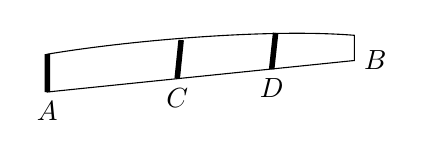
\begin{tikzpicture}[x=1cm,y=1cm]
\draw (0,0) -- (3.9,.4) -- (3.9,.72) .. controls (2.8,.81) and (1,.65) .. (0,.48) -- cycle;
\draw[line width=2pt] (0,0)--(0,.48) (1.65,.17)--(1.7,.66) (2.85,.29)--(2.9,.75);
\node[below] at (0,0){$A$}; \node[below] at (1.65,.17){$C$}; \node[below] at (2.85,.29){$D$}; \node[right] at (3.9,.4){$B$};
\end{tikzpicture}}
OPS $A,B,C,D$ réduits à des points.

\deleted{Ficelle orientée}

\diagram{\begin{tikzcd}[ampersand replacement=\&,column sep=large]
\deleted{A,C,D}\arrow[r,Rightarrow] \& {}\\
\unsure{T|I}\ D,B,C\arrow[r,Rightarrow] \& C,A,D\arrow[r,Rightarrow] \& D,B,C
\end{tikzcd}}
}

\unsure{2}) Être homéom. à $B^n$: On trouve notamment la théorie des décompositions
\figure{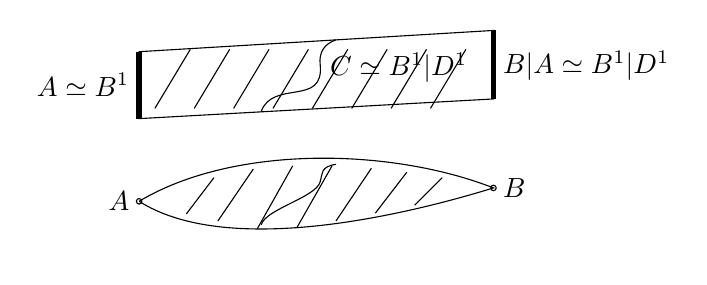
\begin{tikzpicture}[x=1cm,y=1cm]
\draw (0,0)--(4.5,.25)--(4.5,1.12)--(0,.85)--cycle;
\foreach \xa in {.2,.7,1.2,1.7,2.2,2.7,3.2,3.7}{
\draw[thin] (\xa,.13) -- (\xa+.45,.88);}
\draw[line width=2pt] (0,0)--(0,.85) (4.5,.25)--(4.5,1.12);
\draw (1.55,.09) .. controls (1.7,.5) and (2.35,.15) .. (2.3,.68) .. controls (2.28,.84) and (2.35,.95) .. (2.5,1);
\node[left] at (0,.43){$A\simeq B^1$};
\node[right] at (4.5,.67){$\unsure{B|A}\simeq\unsure{B^1|D^1}$};
\node[right] at (2.3,.65){$C\simeq\unsure{B^1|D^1}$};
\begin{scope}[yshift=-1.05cm]
\draw (0,0) .. controls (1.2,.72) and (3.2,.68) .. (4.5,.17) .. controls (3.3,-.2) and (1.1,-.7) .. (0,0);
\foreach \xa/\ya/\xb/\yb in {.6/-.16/.95/.3,1/-.25/1.45/.41,1.5/-.35/1.95/.45,2/-.34/2.45/.45,2.5/-.25/2.95/.42,3/-.15/3.4/.37,3.5/-.05/3.85/.3}
{\draw[thin] (\xa,\ya)--(\xb,\yb);}
\draw (1.55,-.3) .. controls (1.6,-.1) and (2.25,.05) .. (2.3,.25) .. controls (2.33,.35) and (2.3,.44) .. (2.5,.47);
\draw (0,0) circle (.035) (4.5,.17) circle (.035);
\node[left] at (0,0){$A$};\node[right] at (4.5,.17){$B$};
\end{scope}
\end{tikzpicture}}
ou de $I\times B\simeq B^{n+1}$ (avec les deux ``extrémités'' \deleted{$B\times\{0\}$}, $\{0\}\times B^n$, $\{1\}\times B^n$) par des ``lieux'' homéomorphes à $B^{\unsure{n}}$.

\rotatebox{90}{\reflectbox{\unsure{EXTRA STRONG}}}
\rotatebox{90}{\reflectbox{\unsure{EXTRA STRONG}}}
\mspage{12}

\scanpage{14}
\mspage{13}

3) Être homéom. à $S^n$. On trouve p.ex. sur $S^{n+1}$ munie de deux pts \inserted{distincts} (antipodiques, si on veut) $a,b$, une théorie des \unsure{2} décompositions par des $S^n$.

\figure{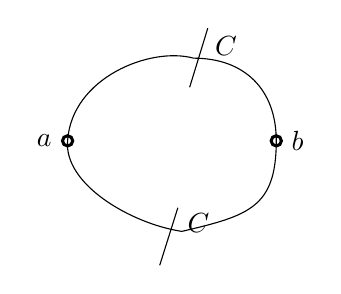
\begin{tikzpicture}[x=1cm,y=1cm]
\draw (0,0) .. controls (.05,.8) and (1.05,1.2) .. (1.6,1.05) .. controls (2.25,1.05) and (2.65,.65) .. (2.65,0) .. controls (2.65,-.85) and (2.3,-.95) .. (1.45,-1.15) .. controls (.8,-1.05) and (-.05,-.55) .. (0,0);
\draw[line width=1.1pt] (0,0) circle (.065) (2.65,0) circle (.065);
\draw (1.55,.68)--(1.78,1.43) (1.17,-1.58)--(1.4,-.85);
\node[left] at (-.08,0){$a$};\node[right] at (2.72,0){$b$};
\node[right] at (1.75,1.2){$C$};\node[right] at (1.4,-1.05){$C$};
\end{tikzpicture}}

On peut aussi exiger, sur un lieu distinct des extrémités, que la structure de $X$ au voisinage de $C$ soit celle de $C\times]-1,1[$, avec $C$ correspondant à $C_0=C\times\{0\}$, et les deux ``rives'' $C\times]-1,0[$, $C\times]0,1[$ étant contenues resp. dans les deux ficelles composantes $X_{A,C}$, $X_{\unsure{B},C}$.

\rotatebox{90}{\reflectbox{\unsure{EXTRA STRONG}}}
\rotatebox{90}{\reflectbox{\unsure{EXTRA STRONG}}}
\mspage{13}

\scanpage{15}
\mspage{14}
\margin{\uline{7 juin}}

2) \uline{Boucle topologique}

\deleted{Soit} \uline{Rives d'une partie} fermée $A$ d'un espace $X$: \deleted{Considérons}

Soit $Z\longmapsto\operatorname{Comp}(Z)=\operatorname{Hom}_{\inserted{\mathrm{cont}}}(Z,\{0,1\})$ \inserted{$=\Gamma(Z,\mathbb F_{2\,Z})$}
(l'ens des parties \inserted{\unsure{clop}} (ouvertes et fermées de $Z$) foncteur contr.variant en $Z$. On pose
\[
\underbrace{\operatorname{Rives}(A,X)}_{\substack{\text{ens des}\\\text{rives de}\\A\text{ dans }X}}
=\underset{\substack{\text{\unsure{Voisinages}}\\\text{de }A\text{ dans }X}}{\lim_{\longrightarrow}}
\operatorname{Comp}(V\setminus A)
=\underset{\unsure{V}}{\lim_{\longrightarrow}}\Gamma(V,i_*(\mathbb F_{2\,U})).
\]
\margin{où $i:U=X\setminus A\hookrightarrow X$ est l'inclusion}

\uline{NB} 1) Supposons que $A$ soit \uline{rég.} immergé, avec voisinage tubulaire: bord $S_{A,X}$. Alors on a
\[
\operatorname{Riv}(A,X)\simeq\operatorname{Comp}(S_{A,X})
\]

2) Supposons que $X$ soit paracompact, alors pour tt faisceau $F$ sur $X$, on a
\[
\Gamma(A,F|A)=\underset{V\in\unsure{\mathcal V}(A,X)}{\lim_{\longrightarrow}}F(V)
\]
\deleted{Alors on a}
Considérons le découpage de $X$ suivant $A$, $(\widetilde X,\widetilde A)$, où
$\widetilde A=\operatorname{Spec}(i_*(\mathbb F_{2\,U}))$, où $i:U=X\setminus A\hookrightarrow X$.
\deleted{\unsure{Donc}} On a $\operatorname{Comp}[\widetilde A]\simeq\Gamma(A,i_*({\unsure{\mathbb F_2}}_{U}))$.

\rotatebox{90}{\reflectbox{\unsure{EXTRA STRONG}}}
\rotatebox{90}{\reflectbox{\unsure{EXTRA STRONG}}}
\mspage{14}

\scanpage{16}
\mspage{15}

application canonique
\[
(*)\qquad \operatorname{Riv}(A,X)\longrightarrow\operatorname{Comp}(\widetilde A)
\]
qui est \inserted{injective, et} \uline{bijective} si $X$ paracompact.
Donc dans ce cas, choisir une rive, c'est choisir un composant de $\widetilde A$.

\uline{NB} L'ens des \deleted{composants}\inserted{rives} de \deleted{$X$} $A$ dans $X$ est une $\mathbb F_2$-algèbre \inserted{comm.} idempotente ($E^2=E$: $\forall E\in\operatorname{Riv}$) avec unité, l'application précédente est un hom. d'alg. unitaires.

Une \uline{birive} \inserted{de $A$ dans $X$} est une \uline{paire} \inserted{$\{\rho,\rho'\}$} d'éléments de $\operatorname{Riv}(A)$, telle que
\[
\rho+\rho'=1
\]
\margin{\uline{NB} Cette algèbre $\operatorname{Riv}$ est nulle ssi $A$ est ouvert, \unsure{en $=$ temps que} fermé.}
\margin{(c'est-à-dire une ``décomposition en 2 composants de $X\setminus A$ au vois. de $A$''}

\deleted{\unsure{Ceci doit être}} (ce qui implique, si $A$ n'est pas ouvert, que $\rho\ne\rho'$).
La birive est triviale si $\{\rho,\rho'\}=\{0,1\}$. On dit que $A$ disconnect $X$ loc.\textsuperscript{t} si $\exists$ birive non triviale.

\deleted{\unsure{Considérons}} Une birive définit $\{\widetilde A_1,\widetilde A_2\}$ telle que $\widetilde A=\widetilde A_1\amalg\widetilde A_2$.
On dit que \deleted{c'est une \unsure{b}} $\{A,\deleted{\{\rho,\rho'\}}\}$

\rotatebox{90}{\reflectbox{\unsure{EXTRA STRONG}}}
\rotatebox{90}{\reflectbox{\unsure{EXTRA STRONG}}}
\mspage{15}

\scanpage{17}
\mspage{16}

définit sur $X$ une structure de \deleted{\uline{boucle topologique}} \uline{maille}, \deleted{dont $A$ est le} \uline{noeud} $A$, si \deleted{$(\widetilde X,\{\widetilde A_1,\widetilde A_2\})$} \deleted{est} $A$ est régulièrement immergé dans $X$ (alors $\widetilde A_{\deleted{\unsure{2}}}$ est régulièrement immergé dans $\widetilde X$, donc $\widetilde A_1$, $\widetilde A_2$ aussi) et si $(\widetilde X,\{\widetilde A_1,\widetilde A_2\})$ satisfait les conditions a) b) c) des ficelles top. (donc est une ficelle top. si $\widetilde A$ est rég. immergé dans $\widetilde X$).
\margin{\unsure{réciproq.}}

Considérons
\[
\widetilde X\amalg_{\widetilde A_1}(\widetilde A_1\longrightarrow A)
\amalg_{\widetilde A_2}(\widetilde A_2\longrightarrow A),
\]
on trouve un espace $\overline X=\operatorname{Dec}_{\beta}(A,X)$, avec deux parties (indexées par $\beta$). can. isom. à $A$, $\{A_\rho,A_{\rho'}\}$, \deleted{\unsure{A}} i.e. une partie isom. à $A\times\beta$
\margin{$\beta=\{\rho,\rho'\}$ la birive}
\diagram{\begin{tikzcd}[ampersand replacement=\&]
\overline X\arrow[r]\&X
\end{tikzcd}}
induisant un isom
\diagram{\begin{tikzcd}[ampersand replacement=\&]
\overline X\setminus\{\underbrace{A_\rho\cup A_{\rho'}}_{A\times\unsure{\rho|\beta}}\}\arrow[r]\&X\setminus A
\end{tikzcd}}
et des homéom
\[
A_\rho\overset{\sim}{\longrightarrow} A,\qquad A_{\rho'}\simeq A
\]
i.e. la projection can.
\diagram{\begin{tikzcd}[ampersand replacement=\&]
A\times\beta\arrow[r,dash]\&A
\end{tikzcd}}

\rotatebox{90}{\reflectbox{\unsure{EXTRA STRONG}}}
\rotatebox{90}{\reflectbox{\unsure{EXTRA STRONG}}}
\mspage{16}

\scanpage{18}
\mspage{17}

Ceci \unsure{vu|or}, on voit que $(A,\beta)$ définit une structure de maille à \inserted{\uline{un}} \uline{noeud} $A$, à \unsure{birive} $\beta$ \deleted{$\unsure{\epsilon}$}, \unsure{ssi} $(\overline X,\{A_\rho,A_{\rho'}\})$ est une \uline{ficelle} top.

Orienter la maille, c'est par définition orienter la ficelle, i.e. choisir $A_\rho$ ou $A_{\rho'}$, i.e. choisir $\rho$ ou $\rho'$ i.e. une des rives qui constituent la birive.
\margin{\uline{NB} \unsure{Dans tout ce qui précède} \unsure{se réduire au cas} $A_1,A_2$ réduits à un point\ldots}

\deleted{On dit que deux structures de}
Considérons deux \deleted{\unsure{struc}} structures de mailles $(A_1,\underbrace{(\rho_1,\rho'_1)}_{\beta_1})$ et $(A_2,\underbrace{\{\rho_2,\rho'_2\}}_{\beta_2})$ sur $X$.

\figure{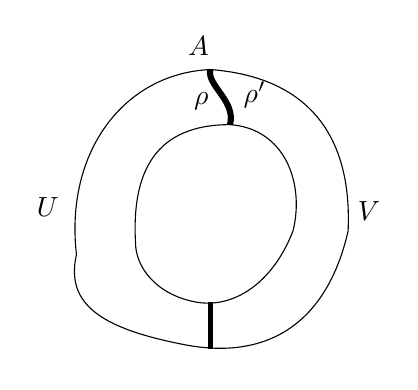
\begin{tikzpicture}[x=1cm,y=1cm]
\draw (0,0) .. controls (-.15,1.3) and (.6,2.3) .. (1.7,2.35) .. controls (3,2.25) and (3.5,1.45) .. (3.45,.3) .. controls (3.2,-.8) and (2.5,-1.35) .. (1.4,-1.15) .. controls (.35,-.95) and (-.15,-.65) .. (0,0);
\draw (.75,.15) .. controls (.7,1.05) and (1,1.65) .. (1.95,1.65) .. controls (2.65,1.6) and (2.9,.9) .. (2.75,.3) .. controls (2.5,-.35) and (2,-.7) .. (1.5,-.6) .. controls (1,-.5) and (.75,-.15) .. (.75,.15);
\draw[line width=2.2pt] (1.7,2.35) .. controls (1.65,2.15) and (2.03,1.95) .. (1.95,1.65);
\draw[line width=1.8pt] (1.7,-.6)--(1.7,-1.2);
\node[above] at (1.55,2.4){$A$};
\node[left] at (1.8,1.95){$\rho$};\node[right] at (2,2.03){$\rho'$};
\node[left] at (-.1,.6){$U$};\node[right] at (3.45,.55){$V$};
\end{tikzpicture}}

Je dis qu'elles sont \deleted{\uline{\unsure{équivalentes}}} \deleted{compatibles} \uline{\unsure{comparables|compatibles}} \deleted{\unsure{compatibles}} si
\deleted{a) $A\cap B$}

a) $A_1\cap A_2=\varnothing$ donc $A_2$ \deleted{définit} \inserted{s'identifie à} une partie de $\overline X^{(A_1,\beta_1)}\setminus A_1\times\beta_1$.

\deleted{b) $A_2$ Si}
b) $A_2$ est un \uline{lieu} de \inserted{$\overline X^{(A_1,\beta_1)}$}

c) Si $U,V$ sont les deux composantes connexes de
$\overline X^{(A_1,\beta_1)}\setminus((A_1,\rho_1)\cup A_1,\rho'_1)\unsure{\setminus|\ne}A_2$,

\rotatebox{90}{\reflectbox{\unsure{EXTRA STRONG}}}
\rotatebox{90}{\reflectbox{\unsure{EXTRA STRONG}}}
\mspage{17}

\scanpage{19}
\mspage{18}

alors $\{U,V\}$ définit à la fois \deleted{$\unsure{\beta_2}$} $\beta_1$, et $\beta_2$.
Je dis que cette condition est en fait symétrique en les deux noeud $(A_i,\beta_i)$.

\rotatebox{90}{\reflectbox{\unsure{EXTRA STRONG}}}

\rotatebox{90}{\reflectbox{\unsure{EXTRA STRONG}}}
\mspage{18}
